% =============================================================================
%  Machine Learning for Petroleum Engineers Using Python
%  Módulo 3 · Clase 5: SVM, Pipelines y Validación Honesta --- Gasoductos PHMSA
%  SLB Ecuador | UDLA
%
%  Compilar: pdflatex -shell-escape presentacion.tex (x2 para refs)
% =============================================================================
\documentclass[aspectratio=169, 11pt]{beamer}

% ── Codificación y lenguaje ──────────────────────────────────────────────────
\usepackage[T1]{fontenc}
\usepackage[utf8]{inputenc}
\usepackage[spanish,es-noshorthands]{babel}

% ── Fuentes ──────────────────────────────────────────────────────────────────
\usepackage{FiraSans}
\usepackage{FiraMono}
\renewcommand{\familydefault}{\sfdefault}

% ── Gráficos y diagramas ────────────────────────────────────────────────────
\usepackage{graphicx}
\usepackage{tikz}
\usetikzlibrary{arrows.meta, positioning, shapes.geometric, calc, fit, decorations.pathreplacing}
\usepackage{fontawesome5}

% ── Código fuente ────────────────────────────────────────────────────────────
\usepackage{minted}
\usepackage{tcolorbox}
\tcbuselibrary{minted, skins, breakable}

% ── Tablas y utilidades ──────────────────────────────────────────────────────
\usepackage{amsmath}
\usepackage{colortbl}
\usepackage{booktabs}
\usepackage{multicol}
\usepackage{hyperref}
\usepackage{calc}

% =============================================================================
%  PALETA DE COLORES (rojo UDLA + variantes)
% =============================================================================
\definecolor{arcaRed}{HTML}{C82B40}
\definecolor{arcaDark}{HTML}{6B1525}
\definecolor{udlaCrimson}{HTML}{A31545}
\definecolor{arcaGray}{HTML}{F5F5F5}
\definecolor{arcaLightGray}{HTML}{EBEBEB}
\definecolor{textDark}{HTML}{2D2D2D}
\definecolor{textMuted}{HTML}{6B7280}
\definecolor{codeGreen}{HTML}{16A34A}
\definecolor{codeBlue}{HTML}{2563EB}
\definecolor{codeOrange}{HTML}{EA580C}
\definecolor{slbBlue}{HTML}{0014DC}
\definecolor{terminalBg}{HTML}{0F172A}
\definecolor{terminalGreen}{HTML}{86EFAC}
\definecolor{terminalMuted}{HTML}{94A3B8}
\definecolor{codeBg}{HTML}{FAFAFA}

% =============================================================================
%  CONFIGURACIÓN DEL TEMA BEAMER
% =============================================================================
\usetheme{default}
\usecolortheme{default}

\setbeamertemplate{navigation symbols}{}
\setbeamertemplate{footline}{}
\setbeamertemplate{headline}{}

\setbeamercolor{normal text}{fg=textDark}
\setbeamercolor{frametitle}{fg=arcaRed, bg=white}
\setbeamercolor{title}{fg=white}
\setbeamercolor{subtitle}{fg=white!85}
\setbeamercolor{author}{fg=white!80}
\setbeamercolor{date}{fg=white!70}
\setbeamercolor{item}{fg=arcaRed}
\setbeamercolor{subitem}{fg=arcaDark}
\setbeamercolor{block title}{fg=white, bg=arcaRed}
\setbeamercolor{block body}{fg=textDark, bg=arcaGray}
\setbeamercolor{block title alerted}{fg=white, bg=codeOrange}
\setbeamercolor{block body alerted}{fg=textDark, bg=arcaGray}
\setbeamercolor{block title example}{fg=white, bg=codeGreen}
\setbeamercolor{block body example}{fg=textDark, bg=arcaGray}
\setbeamercolor{section in toc}{fg=arcaDark}

\setbeamerfont{frametitle}{size=\Large, series=\bfseries}
\setbeamerfont{title}{size=\huge, series=\bfseries}
\setbeamerfont{subtitle}{size=\large}
\setbeamerfont{author}{size=\normalsize}
\setbeamerfont{date}{size=\small}
\setbeamerfont{block title}{size=\normalsize, series=\bfseries}
\setbeamerfont{footnote}{size=\tiny}

\setbeamertemplate{itemize item}{\scriptsize\raise1.5pt\hbox{\color{arcaRed}$\blacktriangleright$}}
\setbeamertemplate{itemize subitem}{\scriptsize\raise1pt\hbox{\color{arcaDark}$\bullet$}}
\setbeamertemplate{enumerate items}[default]
\setbeamercolor{enumerate item}{fg=arcaRed}

% =============================================================================
%  HEADER
% =============================================================================
\setbeamertemplate{headline}{%
  \begin{tikzpicture}[remember picture, overlay]
    \fill[arcaDark] (current page.north west) rectangle
      ([yshift=-0.7cm]current page.north east);
    \node[anchor=west, inner sep=0pt] at
      ([xshift=0.6cm, yshift=-0.35cm]current page.north west)
      {
\includegraphics[height=0.45cm]{../logo_udla_white.png}};
    \node[anchor=east, inner sep=0pt] at
      ([xshift=-0.6cm, yshift=-0.35cm]current page.north east)
      {
\includegraphics[height=0.42cm]{../SLB_white.png}};
  \end{tikzpicture}%
  \vspace{0.7cm}%
}

% =============================================================================
%  FOOTER
% =============================================================================
\setbeamertemplate{footline}{%
  \begin{tikzpicture}[remember picture, overlay]
    \draw[arcaLightGray, line width=0.4pt]
      ([yshift=0.55cm, xshift=0.6cm]current page.south west) --
      ([yshift=0.55cm, xshift=-0.6cm]current page.south east);
    \node[anchor=south, font=\tiny\color{textMuted}] at
      ([yshift=0.15cm]current page.south)
      {Machine Learning for Petroleum Engineers Using Python \(\cdot\) SLB Ecuador};
    \node[anchor=south east, font=\scriptsize\bfseries\color{arcaRed}] at
      ([xshift=-0.6cm, yshift=0.15cm]current page.south east)
      {\insertframenumber};
  \end{tikzpicture}%
}

% =============================================================================
%  FRAMETITLE personalizado con línea roja
% =============================================================================
\setbeamertemplate{frametitle}{%
  \vspace{0.25cm}%
  \usebeamerfont{frametitle}\usebeamercolor[fg]{frametitle}\insertframetitle%
  \par\vspace{2pt}%
  \begin{tikzpicture}
    \fill[arcaRed] (0,0) rectangle (3cm, 1.5pt);
    \fill[arcaLightGray] (3cm,0) rectangle (\textwidth, 0.5pt);
  \end{tikzpicture}%
  \vspace{0.1cm}%
}

% =============================================================================
%  ESTILO DE BLOQUES DE CÓDIGO (minted + tcolorbox)
% =============================================================================
\newtcblisting{pyblock}[1][]{%
  listing engine=minted,
  minted language=python,
  minted style=xcode,
  minted options={
    fontsize=\small,
    linenos=false,
    breaklines=true,
    python3=true
  },
  enhanced,
  colback=codeBg,
  colframe=arcaRed,
  left=8pt,
  right=6pt,
  top=5pt,
  bottom=5pt,
  boxrule=0pt,
  leftrule=3pt,
  arc=3pt,
  listing only,
  title={\hspace{-2pt}\faPython\hspace{5pt}Python},
  fonttitle=\scriptsize\bfseries,
  colbacktitle=arcaRed,
  coltitle=white,
  attach boxed title to top left={xshift=8pt, yshift=-7pt},
  boxed title style={
    arc=2pt, boxrule=0pt,
    top=1.5pt, bottom=1.5pt, left=6pt, right=6pt
  },
  drop fuzzy shadow=black!12,
  #1
}

\newtcblisting{outputblock}[1][]{%
  listing engine=minted,
  minted language=text,
  minted style=bw,
  minted options={
    fontsize=\small,
    breaklines=true,
    formatcom=\color{terminalGreen}
  },
  enhanced,
  colback=terminalBg,
  colframe=terminalBg,
  coltext=terminalGreen,
  left=10pt, right=6pt, top=5pt, bottom=5pt,
  boxrule=0pt,
  arc=3pt,
  listing only,
  title={\hspace{-2pt}\faTerminal\hspace{5pt}Output},
  fonttitle=\scriptsize\bfseries,
  colbacktitle=terminalGreen!85!black,
  coltitle=terminalBg,
  attach boxed title to top left={xshift=8pt, yshift=-7pt},
  boxed title style={
    arc=2pt, boxrule=0pt,
    top=1.5pt, bottom=1.5pt, left=6pt, right=6pt
  },
  #1
}

% =============================================================================
%  SECTION DIVIDERS
% =============================================================================
\newcommand{\sectionframe}[2]{%
  \begingroup
    \setbeamertemplate{headline}{}
    \setbeamertemplate{footline}{}
    \setbeamertemplate{navigation symbols}{}
    \begin{frame}[plain, noframenumbering]
      \begin{tikzpicture}[remember picture, overlay]
        \fill[arcaRed] (current page.south west) rectangle (current page.north east);
        \node[anchor=center, text=white, font=\Huge\bfseries, text width=15cm,
              align=center] at ([yshift=0.5cm]current page.center)
              {\hyphenpenalty=10000\exhyphenpenalty=10000 #1};
        \node[anchor=center, text=white!80, font=\large, text width=10cm,
              align=center] at ([yshift=-0.8cm]current page.center) {#2};
      \end{tikzpicture}
    \end{frame}
  \endgroup
}

% =============================================================================
%  METADATOS
% =============================================================================
\title{Machine Learning for Petroleum Engineers\\Using Python}
\subtitle{Módulo 3 · Clase 5: SVM, Pipelines y Validación Honesta}
\author{Carlos Enrique Mosquera Trujillo}
\date{2026}

% =============================================================================
%  DOCUMENTO
% =============================================================================
% =============================================================================
%  DOCUMENTO
% =============================================================================
\begin{document}
% ── PORTADA ──────────────────────────────────────────────────────────────────
{
\setbeamertemplate{headline}{}
\setbeamertemplate{footline}{}
\begin{frame}[plain, noframenumbering]
  \begin{tikzpicture}[remember picture, overlay]
    \fill[white] (current page.south west) rectangle (current page.north east);
    \fill[arcaRed] (current page.north west) rectangle ([yshift=-0.35cm]current page.north east);
    \fill[arcaDark] (current page.south west) rectangle ([yshift=0.35cm]current page.south east);
    \fill[arcaRed]
      ([xshift=1.1cm, yshift=-0.35cm]current page.north west) rectangle
      ([xshift=1.15cm, yshift=0.35cm]current page.south west);
    \node[anchor=north west, inner sep=0pt] at
      ([xshift=1.8cm, yshift=-1.2cm]current page.north west)
      {
\includegraphics[height=1.6cm]{../logo_udla.png}};
    \node[anchor=north east, inner sep=0pt] at
      ([xshift=-1.5cm, yshift=-1.2cm]current page.north east)
      {
\includegraphics[height=1.5cm]{../SLB.png}};
    \node[anchor=center, text=arcaDark, text width=14.5cm, align=center] at
      ([yshift=0.95cm]current page.center) {
        {\LARGE\bfseries Machine Learning for Petroleum Engineers}\\[8pt]
        {\LARGE\bfseries Using Python}
      };
    \fill[arcaRed]
      ([yshift=-0.35cm, xshift=-3.2cm]current page.center) rectangle
      ([yshift=-0.28cm, xshift=3.2cm]current page.center);
    \node[anchor=center, text=arcaRed, font=\large, text width=13cm, align=center] at
      ([yshift=-1.3cm]current page.center) {
        Módulo 3 · Clase 5\\[3pt]
        SVM, Pipelines y Validación Honesta --- Cierre del Módulo
      };
    \node[anchor=center, text=textMuted, font=\normalsize] at
      ([yshift=-2.5cm]current page.center) {
        {\color{arcaRed}\faUser}\hspace{6pt}Carlos Enrique Mosquera Trujillo
        \hspace{16pt}
        {\color{arcaRed}\faIndustry}\hspace{4pt}SLB Ecuador
      };
  \end{tikzpicture}
\end{frame}
}

% ── RECAP + RUTA ─────────────────────────────────────────────────────────────
\begin{frame}[shrink=8]{Dónde Estamos: la Última Clase del Módulo}
  \vspace{-4pt}
  \begin{columns}[T]
    \begin{column}{0.48\textwidth}
      {\small\color{arcaDark}\bfseries\faCheckCircle\hspace{5pt}Ya saben:}
      \vspace{4pt}
      {\footnotesize\color{textMuted}
      \begin{itemize}\setlength{\itemsep}{3pt}
        \item[{\color{codeGreen}\scriptsize\faCheck}]
          Predecir un \textbf{número} y una \textbf{etiqueta} (C1--C2)
        \item[{\color{codeGreen}\scriptsize\faCheck}]
          Árboles y \textbf{Random Forest} (C3)
        \item[{\color{codeGreen}\scriptsize\faCheck}]
          Multiclase, codificar, imputar, \texttt{GridSearchCV} (C4)
        \item[{\color{codeGreen}\scriptsize\faCheck}]
          Métricas + \textbf{costo de negocio}, siempre
      \end{itemize}
      }
      \vspace{6pt}
      {\scriptsize\color{textMuted}\itshape
        Y traemos una deuda anotada desde la Clase 2:
        validar con \textbf{pozos completos por fuera}. Hoy se paga.}
    \end{column}
    \begin{column}{0.48\textwidth}
      {\small\color{arcaDark}\bfseries\faForward\hspace{5pt}Hoy:}
      \vspace{4pt}
      {\footnotesize\color{textMuted}
      \begin{itemize}\setlength{\itemsep}{3pt}
        \item[{\color{arcaRed}\scriptsize\faArrowRight}]
          Un problema nuevo: \textbf{integridad de ductos} (con fuego incluido)
        \item[{\color{arcaRed}\scriptsize\faArrowRight}]
          El último modelo del módulo: \textbf{SVM} y el \textbf{kernel trick}
        \item[{\color{arcaRed}\scriptsize\faArrowRight}]
          \textbf{Pipelines}: el tubo que ordena todo el flujo
        \item[{\color{arcaRed}\scriptsize\faStar}]
          \textbf{Validación honesta} y \textbf{SMOTE} para clases raras
      \end{itemize}
      }
      \vspace{4pt}
      {\scriptsize\color{arcaDark}\itshape
        Al final: el marcador y el \textbf{mapa de modelos}
        de todo el módulo.}
    \end{column}
  \end{columns}
\end{frame}

% ═════════════════════════════════════════════════════════════════════════════
\sectionframe{Integridad de Ductos}{Un problema nuevo: ya no preguntamos qué roca es --- preguntamos qué se va a romper}
% ═════════════════════════════════════════════════════════════════════════════

% ── ANDRAGOGÍA ───────────────────────────────────────────────────────────────
\begin{frame}[shrink=8]{Ustedes Ya Hacen Esto}
  \vspace{-4pt}
  {\small\color{arcaDark}\bfseries
    Piensen en el ingeniero de integridad de cualquier operadora con líneas de flujo.}

  \vspace{8pt}
  \begin{columns}[T]
    \begin{column}{0.48\textwidth}
      \begin{tcolorbox}[colback=arcaGray, colframe=arcaRed, boxrule=0pt, leftrule=3pt,
        arc=3pt, left=6pt, right=6pt, top=5pt, bottom=5pt]
        {\scriptsize\color{arcaRed}\bfseries\faTools\hspace{4pt}SU PROBLEMA DIARIO}\\[4pt]
        {\scriptsize\color{textMuted}
          Tiene \textbf{cientos de kilómetros} de línea y presupuesto para
          inspeccionar \textbf{unos pocos}. ¿Cuáles primero? Decide mirando:
          edad, recubrimiento, presión, historial\ldots\\[3pt]
          Es decir: decide \textbf{comparando con fallas pasadas}.}
      \end{tcolorbox}
    \end{column}
    \begin{column}{0.48\textwidth}
      {\footnotesize\color{textMuted}
      \begin{itemize}\setlength{\itemsep}{5pt}
        \item[{\color{arcaRed}\scriptsize\faArrowRight}]
          Eso es exactamente un problema de \textbf{clasificación}:
          dadas las características de una línea, ¿qué tipo de falla
          es la más probable?
        \item[{\color{arcaRed}\scriptsize\faArrowRight}]
          Hoy lo haremos con \textbf{fallas reales}: cada incidente
          reportado al regulador de EE.\,UU.\ trae la causa investigada
          \textbf{y el costo en dólares}.
        \item[{\color{codeGreen}\scriptsize\faCheck}]
          Dos preguntas de negocio: ¿fue \textbf{corrosión}?
          Y la que quema: ¿qué fugas terminan en \textbf{fuego}?
      \end{itemize}
      }
    \end{column}
  \end{columns}
\end{frame}

% ── EL DATASET ───────────────────────────────────────────────────────────────
\begin{frame}[shrink=8]{El Dataset: Incidentes Reales, Reportados por Ley}
  \vspace{-4pt}
  {\small\color{arcaDark}\bfseries
    PHMSA (el regulador de ductos de EE.\,UU.): toda falla significativa se reporta, se investiga y se publica.}

  \vspace{8pt}
  \begin{columns}[T]
    \begin{column}{0.5\textwidth}
      {\footnotesize\color{textMuted}
      \begin{itemize}\setlength{\itemsep}{5pt}
        \item[{\color{arcaRed}\scriptsize\faDatabase}]
          Incidentes en \textbf{gasoductos de transmisión},
          2010--hoy. Nos quedamos con los que ocurrieron
          \textbf{en la tubería} y tienen reporte completo:
          \textbf{638 incidentes} de \textbf{132 operadores}.
        \item[{\color{arcaRed}\scriptsize\faSearch}]
          Cada uno trae: características físicas de la línea,
          la \textbf{causa investigada}, si hubo \textbf{ignición},
          y el \textbf{costo total en dólares}.
        \item[{\color{codeGreen}\scriptsize\faCheck}]
          Datos públicos del gobierno de EE.\,UU.
          Curados a un CSV liviano, en español, en el repo del curso.
      \end{itemize}
      }
    \end{column}
    \begin{column}{0.46\textwidth}
      \begin{tcolorbox}[colback=arcaGray, colframe=arcaRed, boxrule=0pt, leftrule=3pt,
        arc=3pt, left=6pt, right=6pt, top=5pt, bottom=5pt]
        {\scriptsize\color{arcaDark}\bfseries\faDollarSign\hspace{4pt}EL COSTO ES REAL}\\[4pt]
        {\scriptsize\color{textMuted}
          Incidente mediano por corrosión: \textbf{\$325\,000}.\\[2pt]
          Incidente mediano \textbf{con ignición}: \textbf{\$896\,000}
          --- casi 4 veces el de una fuga sin fuego (\$234\,000).\\[3pt]
          El hilo de costo del módulo, por primera vez,
          \textbf{sin supuestos}: dólares reportados.}
      \end{tcolorbox}
    \end{column}
  \end{columns}
\end{frame}

% ── ACOTAR ───────────────────────────────────────────────────────────────────
\begin{frame}[shrink=8]{Acotar el Problema (Regla de la Casa)}
  \vspace{-4pt}
  {\footnotesize
  \begin{tabular}{@{}p{3.6cm}p{10.2cm}@{}}
    \toprule
    {\color{arcaDark}\bfseries Pregunta de negocio} &
      Dada una línea y sus condiciones: ¿la falla fue \textbf{corrosión}?
      (y después: ¿la fuga terminó en \textbf{ignición}?) \\
    \midrule
    {\color{arcaDark}\bfseries Target} &
      \texttt{CORROSION} (sí/no) --- binario, como en la Clase 2 \\
    \midrule
    {\color{arcaDark}\bfseries Features} &
      6 numéricas (diámetro, edad, presiones, ubicación, costa afuera)
      + \texttt{RECUBRIMIENTO} (categórica \(\to\) one-hot, como en la C4) \\
    \midrule
    {\color{arcaDark}\bfseries Métrica de éxito} &
      accuracy y \textbf{recall de corrosión} --- y validación \textbf{honesta}
      (el tema de hoy) \\
    \midrule
    {\color{arcaDark}\bfseries Récord a batir} &
      el modelo tonto (nunca corrosión): \textbf{62\,\%} \\
    \bottomrule
  \end{tabular}
  }

  \vspace{8pt}
  {\footnotesize\color{textMuted}
  \begin{itemize}\setlength{\itemsep}{3pt}
    \item[{\color{codeGreen}\scriptsize\faCheck}]
      Fíjense: todo lo de la tabla \textbf{ya lo saben hacer}. Lo nuevo de hoy
      es el modelo (SVM), el orden (pipeline) y la honestidad (validación).
  \end{itemize}
  }
\end{frame}

% ── VARIABLES ────────────────────────────────────────────────────────────────
\begin{frame}[shrink=10]{Las Variables, Una a Una}
  \vspace{-4pt}
  {\small\color{arcaDark}\bfseries
    Todas se explican en una línea --- ese fue un criterio para elegir este dataset.}

  \vspace{6pt}
  {\footnotesize
  \begin{tabular}{@{}llp{7.2cm}@{}}
    \toprule
    {\color{arcaDark}\bfseries Columna} & {\color{arcaDark}\bfseries Tipo} &
    {\color{arcaDark}\bfseries Qué es} \\
    \midrule
    \texttt{DIAMETRO\_PULG} & numérica & diámetro de la línea (pulgadas) \\
    \texttt{EDAD\_ANIOS} & numérica & años desde la instalación hasta el incidente \\
    \texttt{PRESION\_MAX\_PSI} & numérica & presión máxima de operación permitida (MOP) \\
    \texttt{PRESION\_INCIDENTE\_PSI} & numérica & presión al momento del incidente \\
    \texttt{RECUBRIMIENTO} & \textbf{categórica} & alquitrán, asfalto, cinta fría, sin recubrimiento\ldots \\
    \texttt{CLASE\_UBICACION} & numérica (1--4) & densidad poblacional alrededor (1 rural \(\to\) 4 urbana) \\
    \texttt{COSTA\_AFUERA} & binaria & ¿la línea es costa afuera? (0/1) \\
    \texttt{CAUSA} / \texttt{IGNICION} & \textbf{targets} & causa investigada; ¿hubo fuego? \\
    \texttt{COSTO\_USD} & informativa & costo total reportado del incidente \\
    \bottomrule
  \end{tabular}
  }

  \vspace{6pt}
  {\scriptsize\color{textMuted}
  \begin{itemize}\setlength{\itemsep}{2pt}
    \item[{\color{arcaRed}\scriptsize\faExclamationTriangle}]
      Hay 2 columnas más en el CSV que \textbf{no} están en esta tabla.
      Son una trampa a propósito --- las veremos en un rato.
  \end{itemize}
  }
\end{frame}

% ── EXPLORACIÓN: CAUSAS ──────────────────────────────────────────────────────
\begin{frame}{Exploración: ¿Por Qué Fallan los Gasoductos?}
  \vspace{-6pt}
  \begin{columns}[T]
    \begin{column}{0.66\textwidth}
      \centering
      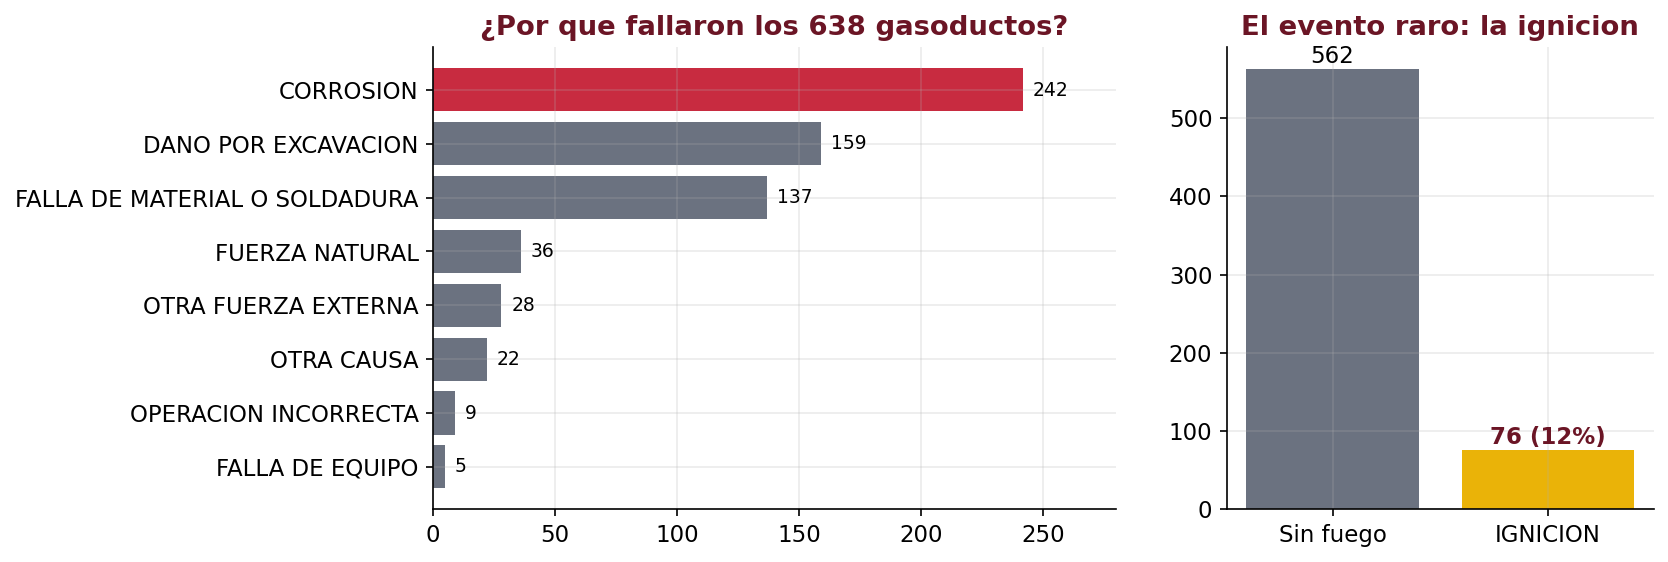
\includegraphics[width=\textwidth]{fig_causas.png}
    \end{column}
    \begin{column}{0.30\textwidth}
      {\footnotesize\color{textMuted}
      \begin{itemize}\setlength{\itemsep}{5pt}
        \item[{\color{arcaRed}\scriptsize\faArrowRight}]
          La \textbf{corrosión} es la causa \#1: 242 de 638
          (\textbf{38\,\%}). Nuestro primer target.
        \item[{\color{arcaRed}\scriptsize\faExclamationTriangle}]
          La \textbf{ignición} es rara: \textbf{12\,\%}.
          Guarden ese número: va a romper un modelo
          más adelante.
        \item[{\color{codeGreen}\scriptsize\faCheck}]
          38\,\% vs 62\,\%: desbalance \textbf{manejable}
          (2 a 1, como la Clase 2).
      \end{itemize}
      }
    \end{column}
  \end{columns}
\end{frame}

% ── EXPLORACIÓN: FÍSICA ──────────────────────────────────────────────────────
\begin{frame}{Exploración: la Física Habla}
  \vspace{-6pt}
  \centering
  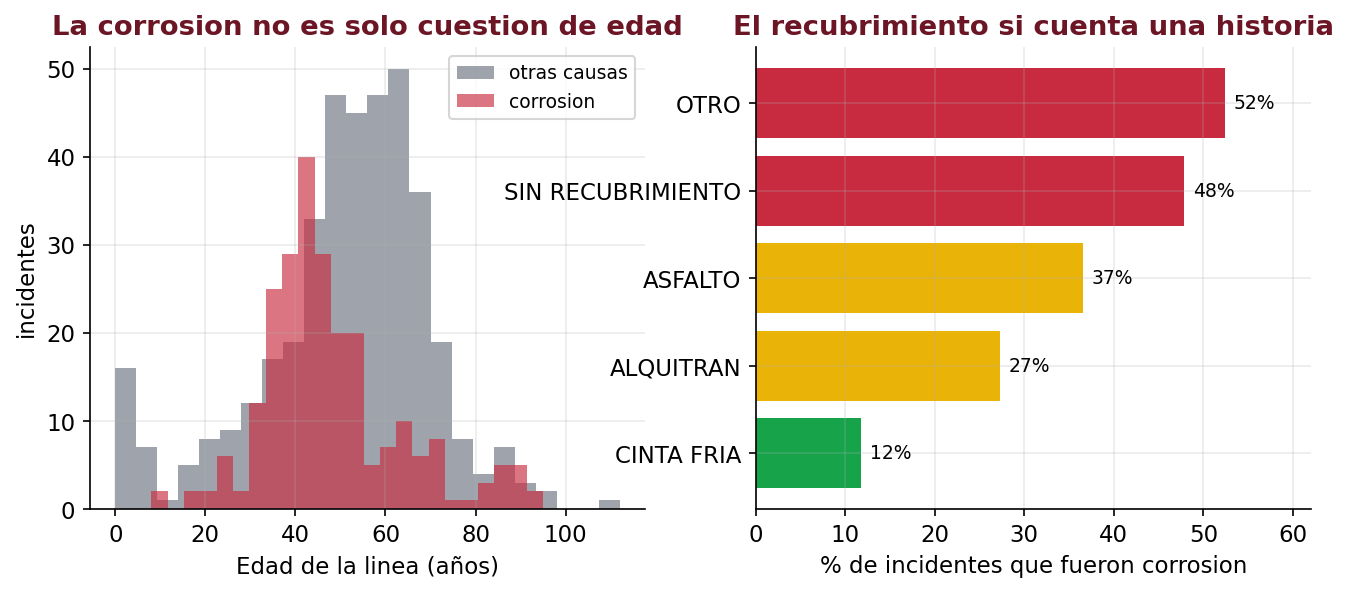
\includegraphics[width=0.92\textwidth]{fig_explora.png}

  \vspace{4pt}
  {\footnotesize\color{textMuted}
  \begin{itemize}\setlength{\itemsep}{3pt}
    \item[{\color{arcaRed}\scriptsize\faArrowRight}]
      Sorpresa: la corrosión \textbf{no} es simplemente ``línea vieja'' ---
      su pico está en los 40 años, y hay líneas de 60+ que fallan por otras causas.
    \item[{\color{codeGreen}\scriptsize\faCheck}]
      El \textbf{recubrimiento} sí ordena el riesgo: cinta fría \textbf{12\,\%}
      de corrosión, sin recubrimiento \textbf{48\,\%}. La física responde:
      el recubrimiento es la primera barrera anticorrosiva.
    \item[{\color{arcaRed}\scriptsize\faBullseye}]
      Ninguna variable decide sola \(\to\) trabajo para un \textbf{modelo}
      que las combine.
  \end{itemize}
  }
\end{frame}

% ── COLUMNAS TRAMPA ──────────────────────────────────────────────────────────
\begin{frame}[shrink=8]{Las Dos Columnas Trampa (Anótenlas)}
  \vspace{-4pt}
  {\small\color{arcaDark}\bfseries
    El CSV trae dos columnas que se conocen \textbf{después} de investigar la falla.}

  \vspace{8pt}
  \begin{columns}[T]
    \begin{column}{0.48\textwidth}
      \begin{tcolorbox}[colback=arcaGray, colframe=arcaRed, boxrule=0pt, leftrule=3pt,
        arc=3pt, left=6pt, right=6pt, top=5pt, bottom=5pt]
        {\scriptsize\color{arcaRed}\bfseries\faExclamationTriangle\hspace{4pt}LAS TRAMPAS}\\[4pt]
        {\scriptsize\color{textMuted}
          \texttt{GAS\_LIBERADO\_MPCS}: cuánto gas escapó
          --- se mide \textbf{después} de la fuga.\\[3pt]
          \texttt{IND\_CORROSION\_GALVANICA}: lo marca el
          \textbf{investigador} cuando ya determinó que
          hubo corrosión.}
      \end{tcolorbox}
    \end{column}
    \begin{column}{0.48\textwidth}
      {\footnotesize\color{textMuted}
      \begin{itemize}\setlength{\itemsep}{5pt}
        \item[{\color{arcaRed}\scriptsize\faQuestion}]
          Si nuestro objetivo es \textbf{priorizar inspecciones
          antes de que la línea falle}\ldots{} ¿podemos usar
          columnas que solo existen \textbf{después} de la falla?
        \item[{\color{arcaRed}\scriptsize\faBan}]
          No. Sería \textbf{predecir el pasado}. Se llama
          \textbf{fuga de información} y es el error más caro
          del ML industrial.
        \item[{\color{codeGreen}\scriptsize\faCheck}]
          Regla de oro: solo features que se conocían
          \textbf{ANTES} del evento. En un rato lo mediremos
          en vivo.
      \end{itemize}
      }
    \end{column}
  \end{columns}
\end{frame}

% ═════════════════════════════════════════════════════════════════════════════
\sectionframe{SVM: la Carretera Más Ancha}{El último modelo del módulo}
% ═════════════════════════════════════════════════════════════════════════════

% ── MARGEN: ANDRAGOGÍA ───────────────────────────────────────────────────────
\begin{frame}[shrink=14]{Separar Dos Poblados con una Carretera}
  \vspace{-6pt}
  \centering
  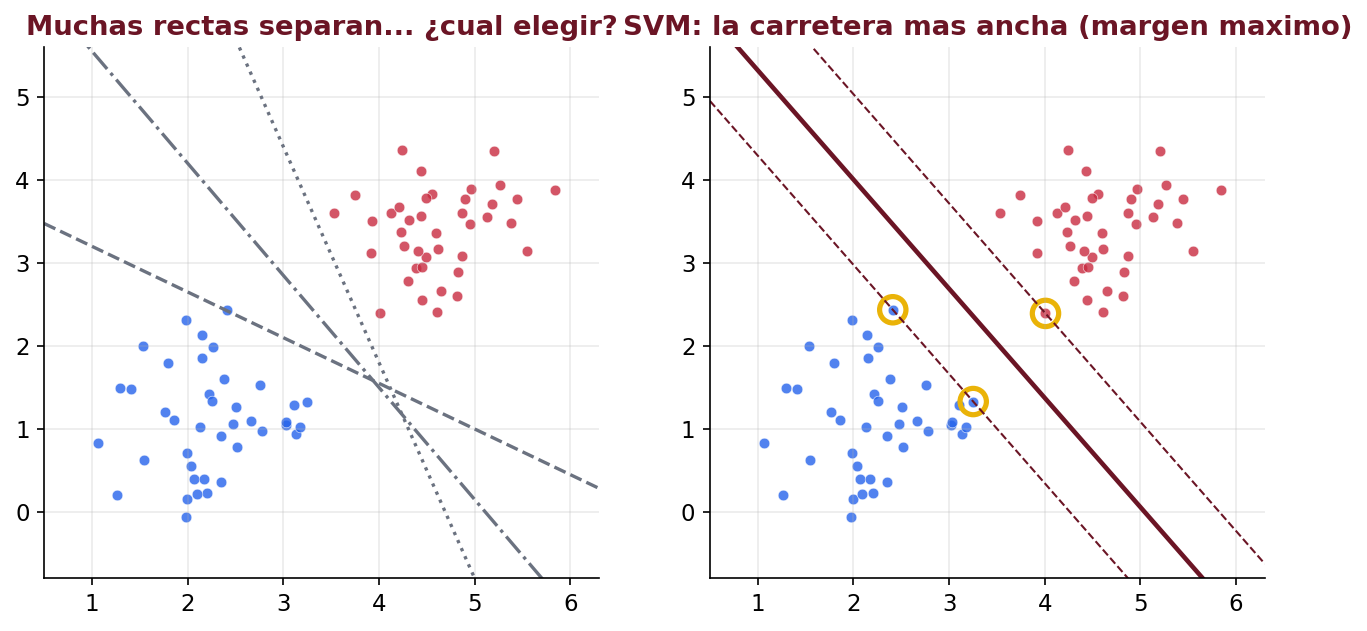
\includegraphics[width=0.95\textwidth]{fig_margen.png}

  \vspace{4pt}
  {\footnotesize\color{textMuted}
  \begin{itemize}\setlength{\itemsep}{3pt}
    \item[{\color{arcaRed}\scriptsize\faArrowRight}]
      Muchas rectas separan los dos grupos (izquierda). La SVM elige la que deja
      \textbf{la carretera más ancha} posible entre los dos poblados (derecha).
    \item[{\color{arcaRed}\scriptsize\faArrowRight}]
      Las casas que \textbf{tocan la cerca} (círculos amarillos) son los
      \textbf{vectores de soporte}: ellas solas definen la carretera.
      Las demás podrían desaparecer y nada cambia.
    \item[{\color{codeGreen}\scriptsize\faCheck}]
      ¿Por qué la más ancha? Porque un dato nuevo, ligeramente distinto,
      \textbf{sigue cayendo del lado correcto}: margen = seguridad.
  \end{itemize}
  }
\end{frame}

% ── SVM EN CÓDIGO (SIN ESCALAR) ──────────────────────────────────────────────
\begin{frame}[fragile,shrink=20]{SVM en Código: el Primer Intento}
  \vspace{-4pt}
  {\small\color{arcaDark}\bfseries
    El patrón de siempre: importar, crear, entrenar, evaluar. Nada nuevo.}

  \vspace{4pt}
  \begin{columns}[T]
    \begin{column}{0.54\textwidth}
      \begin{pyblock}
from sklearn.svm import SVC

svm = SVC()              # el modelo SVM
svm.fit(X_tr, y_tr)      # aprende del train
print(svm.score(X_te, y_te))  # acierto en test
      \end{pyblock}
      \vspace{2pt}
      \begin{outputblock}
0.776
      \end{outputblock}
    \end{column}
    \begin{column}{0.42\textwidth}
      {\scriptsize\color{textMuted}
      \begin{itemize}\setlength{\itemsep}{5pt}
        \item[{\color{codeGreen}\scriptsize\faCheck}]
          \textbf{0.776}: ya le gana al tonto (0.62).
          Cuatro líneas de código.
        \item[{\color{arcaRed}\scriptsize\faQuestionCircle}]
          Pero\ldots{} este modelo mide \textbf{distancias}
          entre incidentes (¿qué tan parecidas son dos líneas?).
        \item[{\color{arcaRed}\scriptsize\faExclamationTriangle}]
          Y nuestras variables tienen \textbf{escalas muy
          distintas}. ¿Cuánto nos está costando eso?
          Siguiente slide.
      \end{itemize}
      }
    \end{column}
  \end{columns}
\end{frame}

% ── EL PROBLEMA DE LA ESCALA ─────────────────────────────────────────────────
\begin{frame}[shrink=14]{El Problema Escondido: las Escalas}
  \vspace{-6pt}
  \centering
  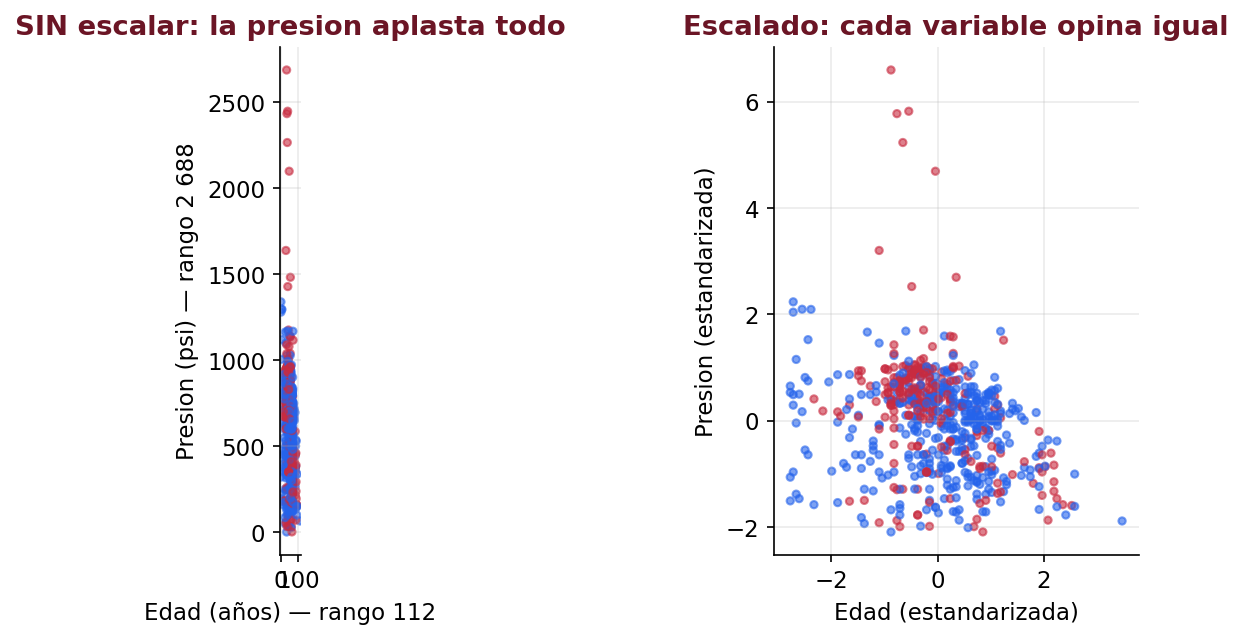
\includegraphics[width=0.88\textwidth]{fig_escala.png}

  \vspace{4pt}
  {\footnotesize\color{textMuted}
  \begin{itemize}\setlength{\itemsep}{3pt}
    \item[{\color{arcaRed}\scriptsize\faArrowRight}]
      La presión se mueve en un rango de \textbf{3\,205 psi}; la edad, en
      \textbf{112 años}; costa afuera, en \textbf{1}. Para una distancia,
      la presión \textbf{grita} y las demás susurran.
    \item[{\color{arcaRed}\scriptsize\faArrowRight}]
      Es ``el paso parejo'' de la Clase 1 otra vez: estandarizar pone a
      \textbf{todas las variables a opinar con la misma voz}.
    \item[{\color{codeGreen}\scriptsize\faCheck}]
      La logística (C2) ya lo necesitaba; los árboles (C3) no;
      la SVM lo necesita \textbf{a gritos}.
  \end{itemize}
  }
\end{frame}

% ═════════════════════════════════════════════════════════════════════════════
\sectionframe{Pipelines: el Tubo}{Escalar bien, sin poder equivocarse}
% ═════════════════════════════════════════════════════════════════════════════

% ── ESCALAR A MANO: LOS 4 PASOS ──────────────────────────────────────────────
\begin{frame}[shrink=8]{Escalar a Mano: 4 Pasos, 2 Errores Clásicos}
  \vspace{-4pt}
  {\small\color{arcaDark}\bfseries
    Así lo hicimos en la Clase 2. Funciona\ldots{} si nadie se equivoca nunca.}

  \vspace{8pt}
  \begin{columns}[T]
    \begin{column}{0.48\textwidth}
      {\footnotesize\color{textMuted}
      \begin{enumerate}\setlength{\itemsep}{5pt}
        \item Ajustar el escalador \textbf{solo con el train}
        \item Transformar el train
        \item Transformar el test \textbf{con el mismo escalador}
        \item Entrenar y evaluar con las versiones escaladas
      \end{enumerate}
      }
      \vspace{6pt}
      {\scriptsize\color{textMuted}\itshape
        Cuatro objetos sueltos (escalador, datos crudos, datos escalados,
        modelo) que hay que coordinar \textbf{a mano}, siempre, sin fallar.}
    \end{column}
    \begin{column}{0.48\textwidth}
      \begin{tcolorbox}[colback=arcaGray, colframe=arcaRed, boxrule=0pt, leftrule=3pt,
        arc=3pt, left=6pt, right=6pt, top=5pt, bottom=5pt]
        {\scriptsize\color{arcaRed}\bfseries\faTimes\hspace{4pt}ERROR CLÁSICO 1}\\[3pt]
        {\scriptsize\color{textMuted}
          Evaluar el test \textbf{sin escalar} (o escalado con otro
          escalador): números basura sin aviso de error.}
      \end{tcolorbox}
      \vspace{6pt}
      \begin{tcolorbox}[colback=arcaGray, colframe=arcaRed, boxrule=0pt, leftrule=3pt,
        arc=3pt, left=6pt, right=6pt, top=5pt, bottom=5pt]
        {\scriptsize\color{arcaRed}\bfseries\faTimes\hspace{4pt}ERROR CLÁSICO 2}\\[3pt]
        {\scriptsize\color{textMuted}
          Ajustar el escalador con \textbf{todos} los datos antes de
          separar train/test: el test se \textbf{filtra} en el
          entrenamiento (fuga, otra vez).}
      \end{tcolorbox}
    \end{column}
  \end{columns}
\end{frame}

% ── QUÉ ES UN PIPELINE ───────────────────────────────────────────────────────
\begin{frame}[shrink=8]{¿Qué es un Pipeline? El Tren de Tratamiento}
  \vspace{-4pt}
  {\small\color{arcaDark}\bfseries
    En sus facilidades el crudo entra crudo y sale listo: separador \(\to\) deshidratador \(\to\) bomba. Nadie carga baldes entre equipos.}

  \vspace{10pt}
  \centering
  \begin{tikzpicture}[node distance=0.55cm]
    \node[draw=textMuted, fill=arcaGray, rounded corners=3pt, minimum height=1.15cm,
          minimum width=2.2cm, align=center, font=\footnotesize] (datos)
          {datos\\\textbf{crudos}};
    \node[draw=codeBlue, fill=arcaGray, rounded corners=3pt, minimum height=1.15cm,
          minimum width=2.9cm, align=center, font=\footnotesize, right=of datos] (esc)
          {\textbf{StandardScaler}\\escala};
    \node[draw=arcaRed, fill=arcaGray, rounded corners=3pt, minimum height=1.15cm,
          minimum width=2.9cm, align=center, font=\footnotesize, right=of esc] (mod)
          {\textbf{SVC}\\clasifica};
    \node[draw=codeGreen, fill=arcaGray, rounded corners=3pt, minimum height=1.15cm,
          minimum width=2.4cm, align=center, font=\footnotesize, right=of mod] (pred)
          {predicción};
    \draw[->, thick, arcaRed] (datos) -- (esc);
    \draw[->, thick, arcaRed] (esc) -- (mod);
    \draw[->, thick, arcaRed] (mod) -- (pred);
    \draw[decorate, decoration={brace, amplitude=6pt, mirror}, arcaDark, thick]
      ([yshift=-3pt]esc.south west) -- ([yshift=-3pt]mod.south east);
    \node[below=0.35cm, font=\scriptsize\bfseries\color{arcaDark}]
      at ($(esc.south)!0.5!(mod.south)$) {el PIPELINE: un solo objeto con .fit() y .predict()};
  \end{tikzpicture}

  \vspace{10pt}
  {\footnotesize\color{textMuted}
  \begin{itemize}\setlength{\itemsep}{3pt}
    \item[{\color{arcaRed}\scriptsize\faArrowRight}]
      Cada pieza hace \textbf{su} paso y le entrega a la siguiente,
      \textbf{en orden, siempre igual}.
    \item[{\color{codeGreen}\scriptsize\faCheck}]
      Al hacer \texttt{.fit()}, el tubo entrena el escalador \textbf{y} el modelo,
      con el train. Al hacer \texttt{.predict()}, escala y clasifica.
      \textbf{Imposible olvidar un paso.}
  \end{itemize}
  }
\end{frame}

% ── PIPELINE EN CÓDIGO ───────────────────────────────────────────────────────
\begin{frame}[fragile,shrink=26]{El Pipeline en Código: 5 Puntos Gratis}
  \vspace{-4pt}
  {\small\color{arcaDark}\bfseries
    El mismo SVM de hace 3 slides --- ahora con el escalado dentro del tubo.}

  \vspace{4pt}
  \begin{columns}[T]
    \begin{column}{0.56\textwidth}
      \begin{pyblock}
from sklearn.pipeline import make_pipeline
from sklearn.preprocessing import StandardScaler

tubo = make_pipeline(
    StandardScaler(),   # paso 1: escalar
    SVC())              # paso 2: clasificar
tubo.fit(X_tr, y_tr)    # el tubo entero aprende
print(tubo.score(X_te, y_te))
      \end{pyblock}
      \vspace{2pt}
      \begin{outputblock}
0.823
      \end{outputblock}
    \end{column}
    \begin{column}{0.40\textwidth}
      {\scriptsize\color{textMuted}
      \begin{itemize}\setlength{\itemsep}{5pt}
        \item[{\color{codeGreen}\scriptsize\faCheck}]
          De 0.776 a \textbf{0.823}: casi \textbf{5 puntos gratis}
          por escalar bien. Sin cambiar el modelo.
        \item[{\color{codeGreen}\scriptsize\faCheck}]
          Y el código quedó \textbf{más corto} que la versión
          manual de 4 pasos.
        \item[{\color{arcaRed}\scriptsize\faArrowRight}]
          \texttt{make\_pipeline} arma el tubo con las piezas
          \textbf{en el orden} en que se las pasan.
      \end{itemize}
      }
    \end{column}
  \end{columns}
\end{frame}

% ── LOS 3 PORQUÉS ────────────────────────────────────────────────────────────
\begin{frame}[shrink=8]{Los 3 Porqués del Pipeline}
  \vspace{-4pt}
  {\small\color{arcaDark}\bfseries
    De aquí en adelante, en este curso, todo modelo que necesite preparación va en pipeline.}

  \vspace{10pt}
  {\footnotesize
  \begin{tabular}{@{}p{0.8cm}p{4.2cm}p{8.6cm}@{}}
    \toprule
    & {\color{arcaDark}\bfseries Porqué} & {\color{arcaDark}\bfseries Qué significa} \\
    \midrule
    {\color{arcaRed}\large\faCut} & \textbf{Código más simple} &
      un solo objeto con \texttt{.fit()} / \texttt{.predict()}; menos variables
      sueltas, menos renglones \\
    \midrule
    {\color{arcaRed}\large\faCheckCircle} & \textbf{Cero olvidos} &
      el test siempre pasa por el \textbf{mismo} tratamiento que el train ---
      los 2 errores clásicos se vuelven imposibles \\
    \midrule
    {\color{arcaRed}\large\faBalanceScale} & \textbf{Validación honesta} &
      cuando hagamos validación cruzada (ya viene), el escalador se reajusta
      \textbf{dentro de cada pliegue} --- sin fugas. A mano, casi nadie lo hace bien \\
    \bottomrule
  \end{tabular}
  }

  \vspace{10pt}
  {\scriptsize\color{arcaDark}\itshape\centering
  El tercero es el importante: el pipeline no es comodidad, es \textbf{honestidad automatizada}.\par}
\end{frame}

% ═════════════════════════════════════════════════════════════════════════════
\sectionframe{El Kernel Trick}{Subir de dimensión para separar lo inseparable}
% ═════════════════════════════════════════════════════════════════════════════

% ── CÍRCULOS: A MANO ─────────────────────────────────────────────────────────
\begin{frame}[shrink=16]{Cuando Ninguna Recta Alcanza}
  \vspace{-6pt}
  \centering
  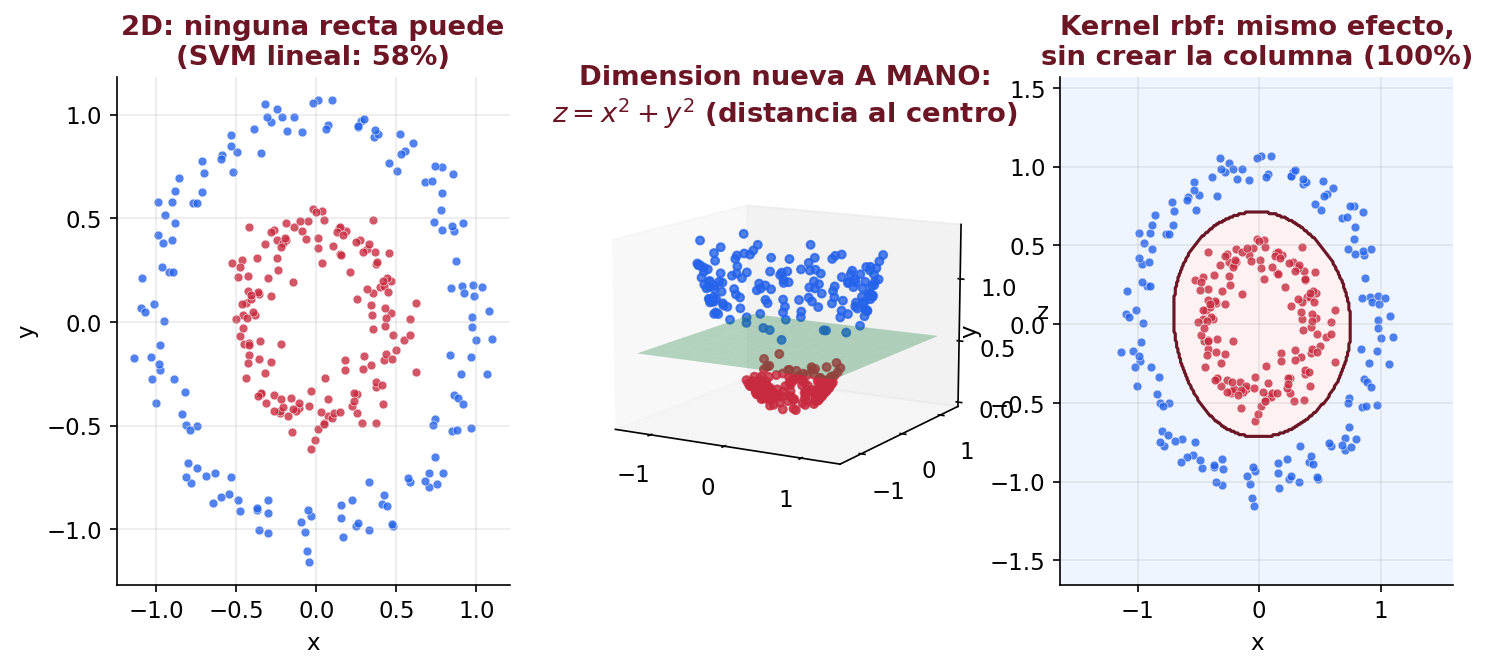
\includegraphics[width=\textwidth]{fig_circulos.png}

  \vspace{4pt}
  {\footnotesize\color{textMuted}
  \begin{itemize}\setlength{\itemsep}{3pt}
    \item[{\color{arcaRed}\scriptsize\faArrowRight}]
      Izquierda: un anillo rodea al centro. La mejor recta se queda en
      \textbf{58\,\%} --- apenas una moneda al aire.
    \item[{\color{codeGreen}\scriptsize\faCheck}]
      Centro: inventamos \textbf{a mano} una columna nueva:
      \(z = x^2 + y^2\) (la \textbf{distancia al centro}). Vista en 3D,
      la nube se separa en dos pisos\ldots{} y un simple \textbf{plano} basta.
    \item[{\color{arcaRed}\scriptsize\faStar}]
      Derecha: el kernel \texttt{rbf} logra \textbf{exactamente el mismo efecto}
      --- \textbf{100\,\%} --- sin que nadie creara la columna. Ese es el truco.
  \end{itemize}
  }
\end{frame}

% ── LA IDEA EN PALABRAS ──────────────────────────────────────────────────────
\begin{frame}[shrink=8]{La Idea en Palabras (Sin Matemática)}
  \vspace{-4pt}
  {\small\color{arcaDark}\bfseries
    Si el problema no se puede separar en el plano\ldots{} míralo desde otra dimensión.}

  \vspace{8pt}
  \begin{columns}[T]
    \begin{column}{0.48\textwidth}
      \begin{tcolorbox}[colback=arcaGray, colframe=arcaRed, boxrule=0pt, leftrule=3pt,
        arc=3pt, left=6pt, right=6pt, top=5pt, bottom=5pt]
        {\scriptsize\color{arcaRed}\bfseries\faLayerGroup\hspace{4pt}SUBIR DE DIMENSIÓN}\\[4pt]
        {\scriptsize\color{textMuted}
          En 2D el anillo es inseparable. Pero al agregar
          ``distancia al centro'', los puntos rojos quedan
          \textbf{abajo} y los azules \textbf{arriba}: un plano
          los separa.\\[3pt]
          Crear la columna correcta \textbf{convierte un problema
          curvo en uno recto}.}
      \end{tcolorbox}
    \end{column}
    \begin{column}{0.48\textwidth}
      {\footnotesize\color{textMuted}
      \begin{itemize}\setlength{\itemsep}{5pt}
        \item[{\color{arcaRed}\scriptsize\faExclamationTriangle}]
          El problema: ¿\textbf{cuál} columna inventar? ¿\(x^2\)?
          ¿\(x \cdot y\)? ¿\(\sqrt{x}\)? Con nuestras \textbf{11 features},
          solo los cuadrados y productos de pares ya son
          \textbf{más de 70 columnas} nuevas. Y quizá se necesiten cientos.
        \item[{\color{arcaRed}\scriptsize\faBolt}]
          \textbf{El kernel trick}: una propiedad matemática de la SVM
          le permite obtener \textbf{el efecto} de todas esas columnas
          \textbf{sin calcular ninguna}.
        \item[{\color{codeGreen}\scriptsize\faCheck}]
          En el código, todo el truco es un argumento:
          \texttt{SVC(kernel='rbf')}. Y es el valor por defecto.
      \end{itemize}
      }
    \end{column}
  \end{columns}
\end{frame}

% ── LAS LUNAS ────────────────────────────────────────────────────────────────
\begin{frame}[shrink=14]{Las Lunas Vuelven (Por Última Vez)}
  \vspace{-6pt}
  \centering
  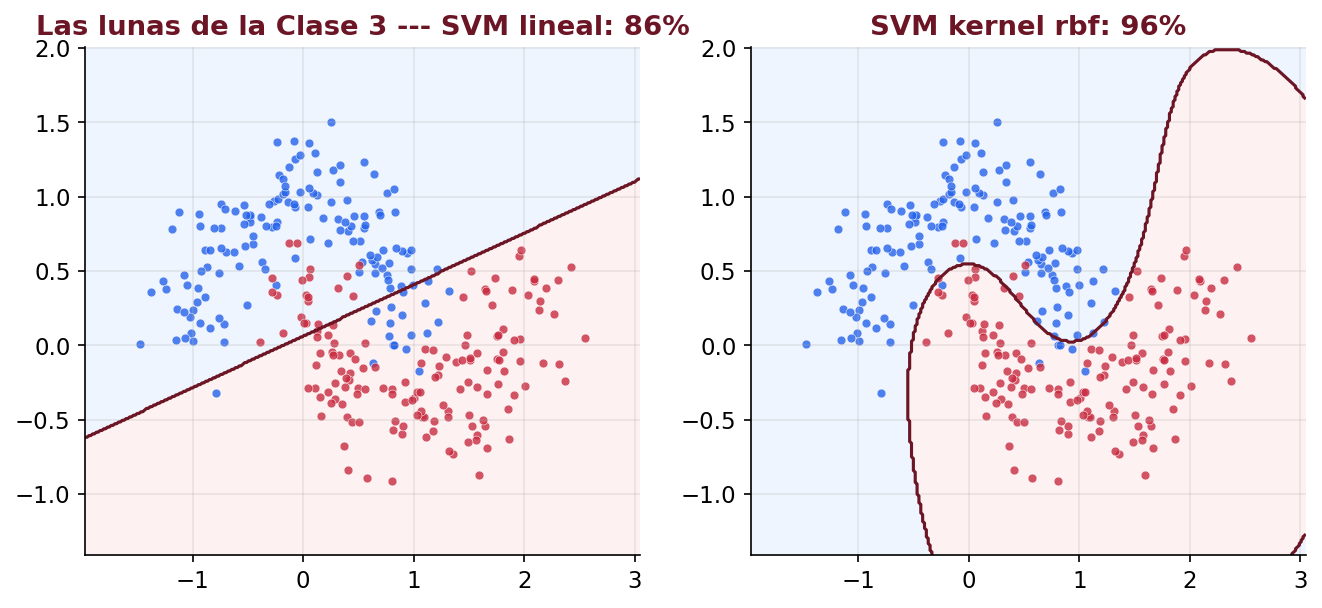
\includegraphics[width=0.9\textwidth]{fig_lunas_svm.png}

  \vspace{4pt}
  {\footnotesize\color{textMuted}
  \begin{itemize}\setlength{\itemsep}{3pt}
    \item[{\color{arcaRed}\scriptsize\faArrowRight}]
      En la Clase 3 las lunas derrotaron a la \textbf{logística} y las salvó
      el \textbf{árbol}. Hoy, la SVM lineal se queda en 86\,\%\ldots
    \item[{\color{codeGreen}\scriptsize\faCheck}]
      \ldots y el kernel \texttt{rbf} dibuja una frontera \textbf{curva y suave}:
      96\,\%. Comparen con los escalones rectos del árbol: dos formas
      distintas de ser no lineal.
  \end{itemize}
  }
\end{frame}

% ── GAMMA ────────────────────────────────────────────────────────────────────
\begin{frame}[shrink=14]{La Perilla gamma: el Radio de Influencia}
  \vspace{-6pt}
  \centering
  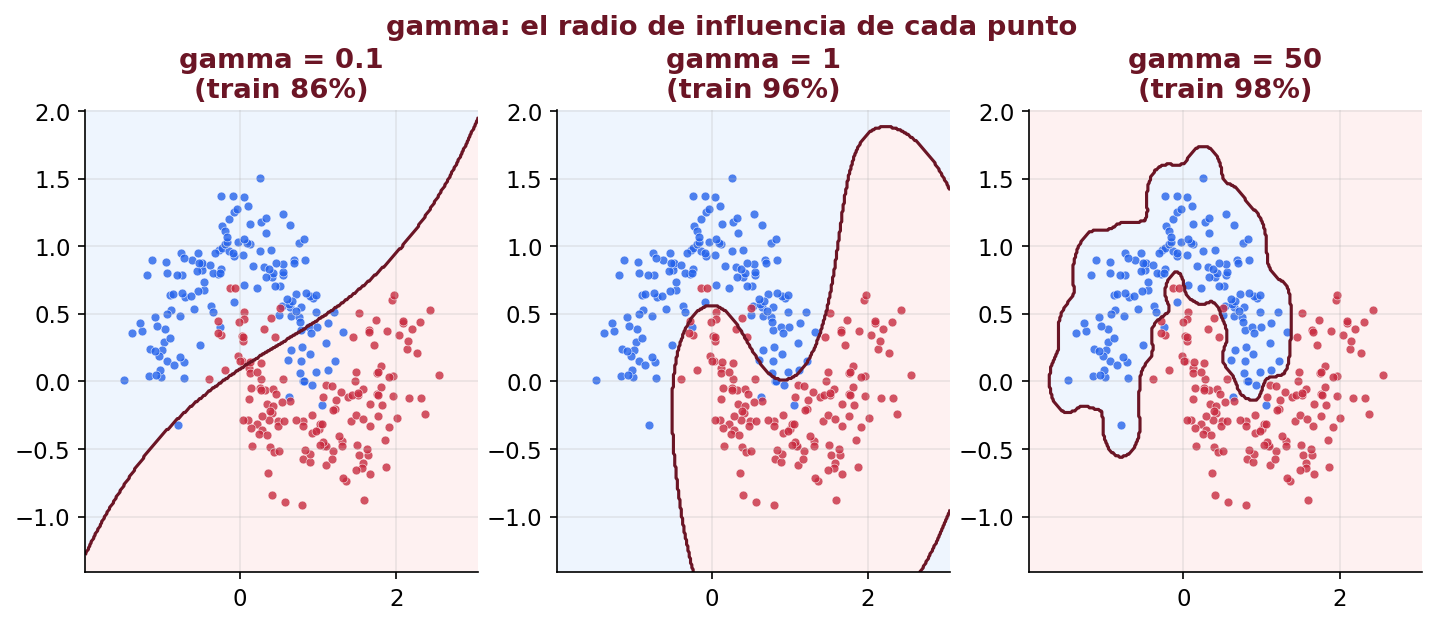
\includegraphics[width=\textwidth]{fig_gamma.png}

  \vspace{4pt}
  {\footnotesize\color{textMuted}
  \begin{itemize}\setlength{\itemsep}{3pt}
    \item[{\color{arcaRed}\scriptsize\faArrowRight}]
      gamma pequeño = cada punto influye \textbf{lejos} \(\to\) frontera suave,
      casi recta. gamma grande = cada punto solo manda \textbf{en su vecindario}
      \(\to\) la frontera se vuelve paranoica y \textbf{encierra puntos sueltos}.
    \item[{\color{arcaRed}\scriptsize\faExclamationTriangle}]
      ¿Train 98\,\% con gamma = 50? Eso ya lo vieron en la C3: huele a
      \textbf{memorizar}, no a aprender. Es el overfitting con otra perilla.
  \end{itemize}
  }
\end{frame}

% ── C ────────────────────────────────────────────────────────────────────────
\begin{frame}[shrink=14]{La Perilla C: ¿Cuánto Castigo por Invadir?}
  \vspace{-6pt}
  \centering
  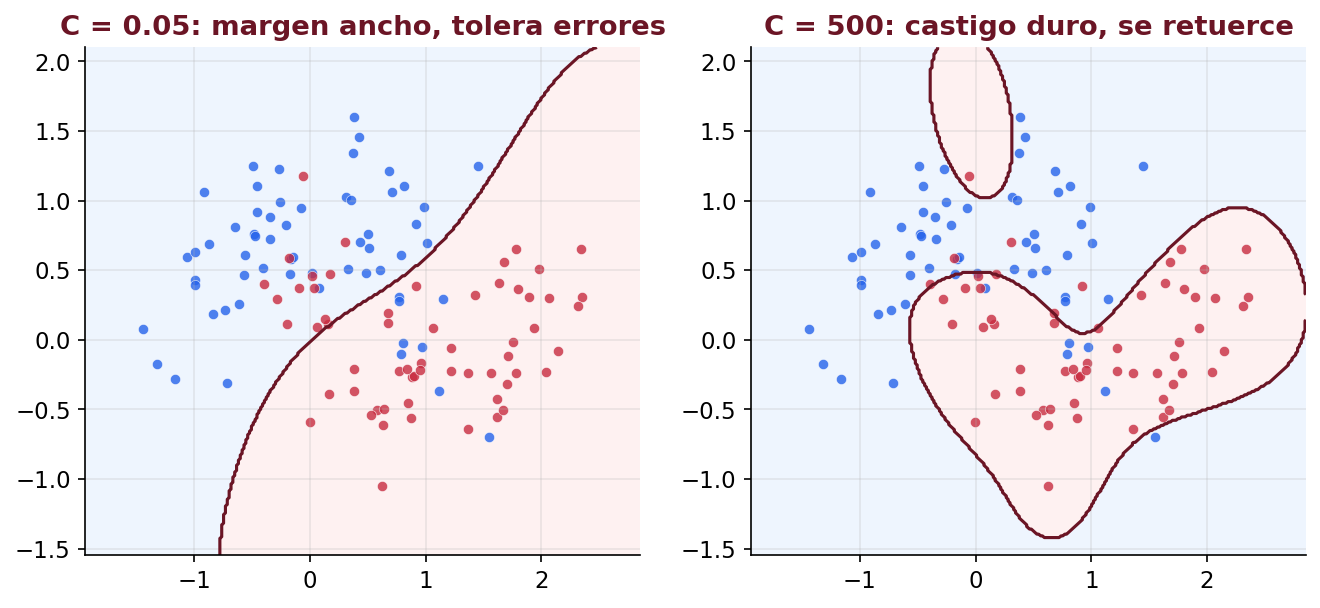
\includegraphics[width=0.9\textwidth]{fig_C.png}

  \vspace{4pt}
  {\footnotesize\color{textMuted}
  \begin{itemize}\setlength{\itemsep}{3pt}
    \item[{\color{arcaRed}\scriptsize\faArrowRight}]
      C chico: carretera \textbf{ancha y tranquila} --- tolera que algunas casas
      queden del lado equivocado. C grande: \textbf{castigo duro} por cada
      invasor --- la carretera se retuerce para no dejar ninguno.
    \item[{\color{arcaRed}\scriptsize\faSlidersH}]
      \texttt{C} y \texttt{gamma} son los \textbf{hiperparámetros} de la SVM
      (¿recuerdan la C4? las perillas que ustedes eligen).
      ¿Y cómo se eligen \textbf{sin hacer trampa}? Sección siguiente.
  \end{itemize}
  }
\end{frame}

% ── EL KERNEL EN LOS DUCTOS ──────────────────────────────────────────────────
\begin{frame}[shrink=10]{¿Y en Nuestros Ductos? La Lección Honesta}
  \vspace{-4pt}
  {\small\color{arcaDark}\bfseries
    Probamos las dos SVM en el problema de corrosión. Miren:}

  \vspace{8pt}
  \centering
  {\footnotesize
  \begin{tabular}{@{}lcc@{}}
    \toprule
    {\color{arcaDark}\bfseries Modelo (siempre en pipeline)} & {\color{arcaDark}\bfseries Accuracy}
      & {\color{arcaDark}\bfseries F1 corrosión} \\
    \midrule
    SVM \textbf{lineal} & \textbf{0.828} & 0.732 \\
    SVM kernel \texttt{rbf} & 0.823 & 0.730 \\
    \bottomrule
  \end{tabular}
  }

  \vspace{12pt}
  {\footnotesize\color{textMuted}
  \begin{itemize}\setlength{\itemsep}{4pt}
    \item[{\color{arcaRed}\scriptsize\faArrowRight}]
      El kernel \textbf{no ganó}: este problema resultó \textbf{casi lineal}.
      Pasa muchísimo con datos tabulares reales.
    \item[{\color{codeGreen}\scriptsize\faCheck}]
      La lección profesional: \textbf{prueben siempre el lineal primero}.
      Es más rápido, más explicable, y a veces empata o gana.
      El kernel es un \textbf{as bajo la manga} (círculos, lunas),
      no un reflejo automático.
    \item[{\color{arcaRed}\scriptsize\faBullseye}]
      Esto también es andragogía de ingeniero: nadie perfora con la broca
      más cara \textbf{si la formación no lo pide}.
  \end{itemize}
  }
\end{frame}

% ═════════════════════════════════════════════════════════════════════════════
\sectionframe{Afinar sin Hacer Trampa}{Validación cruzada, GridSearch y la fuga}
% ═════════════════════════════════════════════════════════════════════════════

% ── CROSS VAL ────────────────────────────────────────────────────────────────
\begin{frame}[fragile,shrink=20]{Una Foto Puede Mentir: 5 Fotos Mienten Menos}
  \vspace{-4pt}
  {\small\color{arcaDark}\bfseries
    Nuestro split train/test es UNA repartición al azar. ¿Y si nos tocó una fácil? ¿O una difícil?}

  \vspace{4pt}
  \begin{columns}[T]
    \begin{column}{0.54\textwidth}
      \begin{pyblock}
from sklearn.model_selection import cross_val_score

notas = cross_val_score(tubo, X, y, cv=5)
print(notas.round(3))   # 5 examenes distintos
print(notas.mean().round(3))
      \end{pyblock}
      \vspace{2pt}
      \begin{outputblock}[]
[0.789 0.781 0.812 0.787 0.764]
0.787
      \end{outputblock}
    \end{column}
    \begin{column}{0.42\textwidth}
      {\scriptsize\color{textMuted}
      \begin{itemize}\setlength{\itemsep}{5pt}
        \item[{\color{arcaRed}\scriptsize\faRedo}]
          \texttt{cv=5}: parte los datos en \textbf{5 pliegues};
          entrena 5 veces, cada vez dejando un pliegue distinto
          como examen. \textbf{Todos los datos examinan una vez.}
        \item[{\color{arcaRed}\scriptsize\faEye}]
          Miren la dispersión: de \textbf{0.764 a 0.812}.
          Una sola foto pudo decirnos cualquiera de esos números.
        \item[{\color{codeGreen}\scriptsize\faCheck}]
          Reportar \textbf{media de 5} \(>\) reportar 1 número
          con suerte. Esto es lo que \texttt{GridSearchCV}
          hacía por dentro en la C4.
      \end{itemize}
      }
    \end{column}
  \end{columns}
\end{frame}

% ── GRIDSEARCH ───────────────────────────────────────────────────────────────
\begin{frame}[fragile,shrink=22]{GridSearch Sobre el Tubo Completo}
  \vspace{-4pt}
  {\small\color{arcaDark}\bfseries
    Novedad de hoy: la parrilla nombra la pieza del tubo --- \texttt{svc\_\_C} = ``la perilla C, de la pieza svc''.}

  \vspace{4pt}
  \begin{columns}[T]
    \begin{column}{0.56\textwidth}
      \begin{pyblock}
from sklearn.model_selection import GridSearchCV

perillas = {'svc__C': [0.1, 1, 10, 100],
            'svc__gamma': [0.01, 0.1, 1]}
buscador = GridSearchCV(tubo, perillas, cv=5)
buscador.fit(X_tr, y_tr)   # 12 combos x 5 pliegues
print('mejor:', buscador.best_params_)
      \end{pyblock}
      \vspace{2pt}
      \begin{outputblock}
mejor: {'svc__C': 1, 'svc__gamma': 0.01}
      \end{outputblock}
    \end{column}
    \begin{column}{0.40\textwidth}
      {\scriptsize\color{textMuted}
      \begin{itemize}\setlength{\itemsep}{5pt}
        \item[{\color{codeGreen}\scriptsize\faCheck}]
          Como el tubo va \textbf{completo} dentro de la búsqueda,
          el escalador se reajusta \textbf{en cada pliegue}:
          cero fugas. (El porqué \#3 del pipeline, cumplido.)
        \item[{\color{arcaRed}\scriptsize\faArrowRight}]
          Con las perillas ganadoras, el test da \textbf{0.828}
          (veníamos de 0.823): mejora fina, sin trampa.
        \item[{\color{arcaRed}\scriptsize\faEye}]
          gamma ganador = \textbf{0.01} (el más suave de la
          parrilla): otra pista de que el problema es casi lineal.
      \end{itemize}
      }
    \end{column}
  \end{columns}
\end{frame}

% ── HEATMAP ──────────────────────────────────────────────────────────────────
\begin{frame}{El Mapa de Perillas Completo}
  \vspace{-6pt}
  \begin{columns}[T]
    \begin{column}{0.52\textwidth}
      \centering
      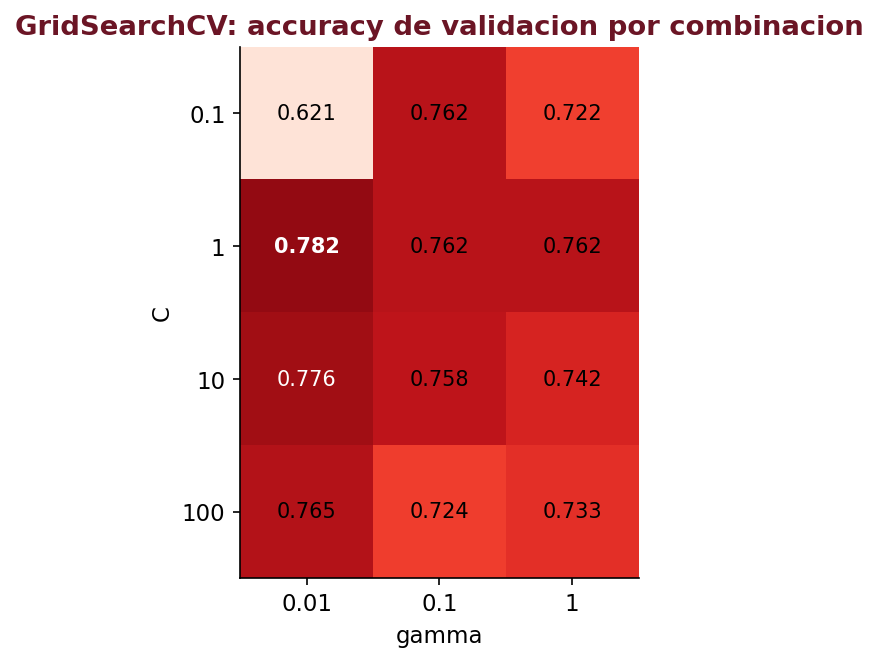
\includegraphics[height=0.72\textheight]{fig_grid_heatmap.png}
    \end{column}
    \begin{column}{0.44\textwidth}
      {\footnotesize\color{textMuted}
      \begin{itemize}\setlength{\itemsep}{5pt}
        \item[{\color{arcaRed}\scriptsize\faArrowRight}]
          Cada casilla = una combinación de perillas, calificada
          con sus \textbf{5 exámenes internos}.
        \item[{\color{codeGreen}\scriptsize\faCheck}]
          La zona buena es \textbf{amplia y estable} (0.76--0.78):
          el modelo no está colgado de una perilla mágica.
          Eso da confianza.
        \item[{\color{arcaRed}\scriptsize\faExclamationTriangle}]
          La esquina C = 0.1 con gamma = 0.01 se desploma (0.62
          = el tonto): castigo tan suave que el modelo
          \textbf{se rinde} y dice siempre ``no corrosión''.
      \end{itemize}
      }
    \end{column}
  \end{columns}
\end{frame}

% ── LA TRAMPA MEDIDA ─────────────────────────────────────────────────────────
\begin{frame}[shrink=10]{La Trampa, Medida en Vivo}
  \vspace{-4pt}
  {\small\color{arcaDark}\bfseries
    ¿Recuerdan las 2 columnas prohibidas? Agreguemos UNA al modelo, ``por curiosidad''.}

  \vspace{10pt}
  \centering
  {\footnotesize
  \begin{tabular}{@{}lc@{}}
    \toprule
    {\color{arcaDark}\bfseries Features} & {\color{arcaDark}\bfseries Accuracy test} \\
    \midrule
    Las 11 honestas (lo que sabías ANTES de la falla) & 0.823 \\
    \rowcolor{arcaGray}
    + \texttt{IND\_CORROSION\_GALVANICA} (del reporte del investigador)
      & {\color{arcaRed}\bfseries 0.906} \\
    \bottomrule
  \end{tabular}
  }

  \vspace{12pt}
  {\footnotesize\color{textMuted}
  \begin{itemize}\setlength{\itemsep}{4pt}
    \item[{\color{arcaRed}\scriptsize\faExclamationTriangle}]
      ¡8 puntos gratis! Pero es un modelo que necesita\ldots{}
      \textbf{que la falla ya haya ocurrido y esté investigada}.
      Inútil para priorizar inspecciones. \textbf{Predice el pasado.}
    \item[{\color{arcaRed}\scriptsize\faBan}]
      Así se ve la \textbf{fuga de información} en la vida real: un número
      espectacular que se derrumba en producción. Si un resultado parece
      demasiado bueno, \textbf{pregunten qué sabía el modelo y cuándo}.
    \item[{\color{codeGreen}\scriptsize\faCheck}]
      Ya la vimos 3 veces en el módulo: escalar antes del split (hoy),
      imputar con todo el dataset (C4), y esta. \textbf{Misma enfermedad,
      tres disfraces.}
  \end{itemize}
  }
\end{frame}

% ── GROUPKFOLD CÓDIGO ────────────────────────────────────────────────────────
\begin{frame}[fragile,shrink=26]{La Pregunta Final: ¿el Modelo Viaja?}
  \vspace{-4pt}
  {\small\color{arcaDark}\bfseries
    Nuestros pliegues mezclan operadores. Pero el negocio pregunta: ¿funciona con un operador NUEVO?}

  \vspace{4pt}
  \begin{columns}[T]
    \begin{column}{0.56\textwidth}
      \begin{pyblock}
from sklearn.model_selection import GroupKFold

notas = cross_val_score(
    tubo, X, y,
    cv=GroupKFold(5),          # pliegues por grupo
    groups=d['OPERADOR_ID'])   # el grupo: operador
print(notas.mean().round(3))
      \end{pyblock}
      \vspace{2pt}
      \begin{outputblock}
0.766
      \end{outputblock}
    \end{column}
    \begin{column}{0.40\textwidth}
      {\scriptsize\color{textMuted}
      \begin{itemize}\setlength{\itemsep}{5pt}
        \item[{\color{arcaRed}\scriptsize\faUsers}]
          \texttt{GroupKFold}: cada pliegue deja \textbf{operadores
          completos} por fuera. El examen es con empresas
          que el modelo \textbf{jamás vio}.
        \item[{\color{codeGreen}\scriptsize\faCheck}]
          0.787 \(\to\) 0.766: cae solo \textbf{2 puntos}.
          Buena noticia: el modelo aprendió física de ductos,
          no mañas de cada operador. \textbf{Viaja.}
        \item[{\color{arcaRed}\scriptsize\faQuestionCircle}]
          ¿Y si hubiéramos hecho esto con las \textbf{facies}
          de la Clase 4, dejando \textbf{pozos} por fuera?
      \end{itemize}
      }
    \end{column}
  \end{columns}
\end{frame}

% ── GROUPKFOLD: LA DEUDA ─────────────────────────────────────────────────────
\begin{frame}{La Deuda del Módulo, Pagada}
  \vspace{-6pt}
  \begin{columns}[T]
    \begin{column}{0.62\textwidth}
      \centering
      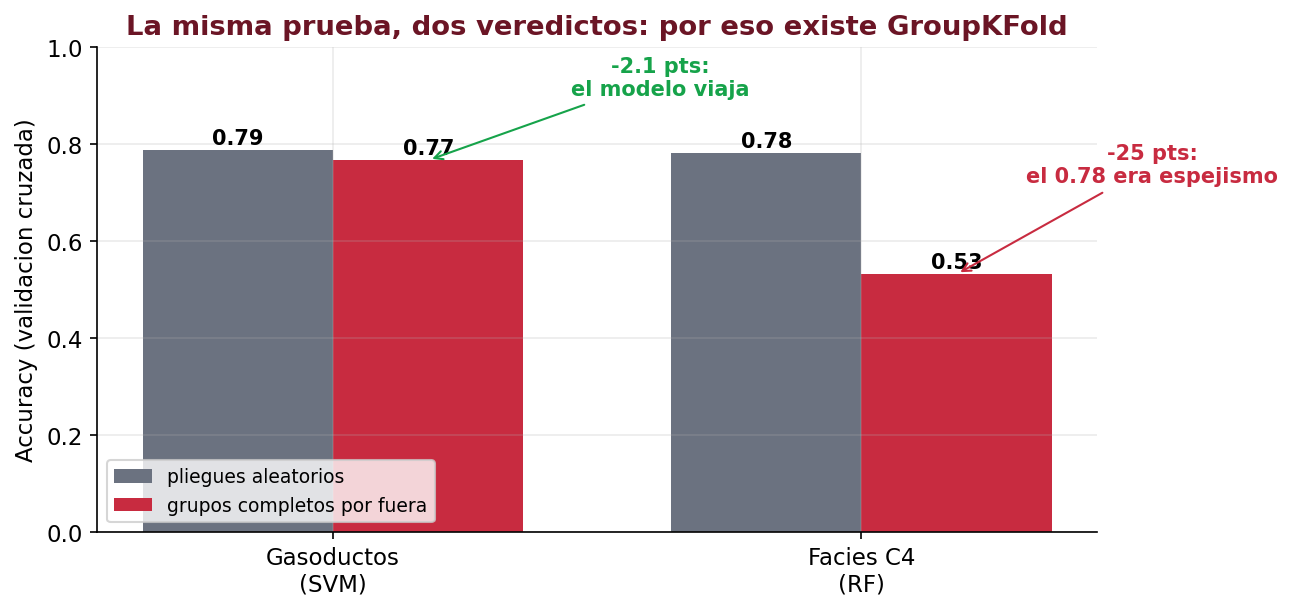
\includegraphics[width=\textwidth]{fig_groupkfold.png}
    \end{column}
    \begin{column}{0.34\textwidth}
      {\footnotesize\color{textMuted}
      \begin{itemize}\setlength{\itemsep}{5pt}
        \item[{\color{arcaRed}\scriptsize\faExclamationTriangle}]
          Las facies: aleatorio \textbf{0.78} \(\to\) pozos por fuera
          \textbf{0.53}. \textbf{25 puntos de espejismo}: medios pies
          vecinos del mismo pozo estaban repartidos entre train y test.
        \item[{\color{arcaRed}\scriptsize\faArrowRight}]
          Esta es la deuda que anotamos en las Clases 2, 3 y 4.
          El 0.76 de facies era real \textbf{solo para pozos ya vistos}.
        \item[{\color{codeGreen}\scriptsize\faCheck}]
          GroupKFold no ``mejora'' el modelo: \textbf{les dice la
          verdad}. A veces certifica (ductos), a veces desinfla
          (facies). Ambas valen oro.
      \end{itemize}
      }
    \end{column}
  \end{columns}
\end{frame}

% ── PRÁCTICA 1 ───────────────────────────────────────────────────────────────
\begin{frame}[shrink=8]{Su Turno: Afinar con Honestidad \hfill {\normalsize\color{arcaRed}\faClock\hspace{4pt}15 min}}
  \vspace{-4pt}
  {\small\color{arcaDark}\bfseries
    Todo con pipeline. Todo sin tocar el test hasta el final.}

  \vspace{8pt}
  {\footnotesize
  \begin{enumerate}\setlength{\itemsep}{7pt}
    \item Armen un pipeline con \texttt{StandardScaler} y \texttt{SVC(kernel='linear')}
      y calculen su \texttt{cross\_val\_score} con \texttt{cv=5}. ¿Confirma que el
      lineal compite con el \texttt{rbf}?
    \item Amplíen la parrilla del \texttt{GridSearchCV} agregando
      \texttt{'svc\_\_kernel': ['linear', 'rbf']}. ¿Quién gana ahora y con qué perillas?
    \item Evalúen su mejor modelo con \texttt{GroupKFold} por operador.
      ¿Cuánto cae respecto a los pliegues aleatorios?
    \item Pregunta de negocio: escriban \textbf{una frase} para el gerente de
      integridad diciendo qué accuracy debe esperar \textbf{y por qué esa}
      (¿la de pliegues aleatorios o la de operadores por fuera?).
  \end{enumerate}
  }
\end{frame}

% ═════════════════════════════════════════════════════════════════════════════
\sectionframe{SMOTE: Fabricar lo Raro}{La segunda pregunta: ¿qué fugas terminan en fuego?}
% ═════════════════════════════════════════════════════════════════════════════

% ── LA IGNICIÓN ──────────────────────────────────────────────────────────────
\begin{frame}[shrink=8]{La Segunda Pregunta de Negocio: el Fuego}
  \vspace{-4pt}
  {\small\color{arcaDark}\bfseries
    Mismo dataset, nuevo target: \texttt{IGNICION}. Solo el 12\,\% de las fugas se encienden.}

  \vspace{8pt}
  \begin{columns}[T]
    \begin{column}{0.48\textwidth}
      {\footnotesize\color{textMuted}
      \begin{itemize}\setlength{\itemsep}{5pt}
        \item[{\color{arcaRed}\scriptsize\faDollarSign}]
          ¿Por qué importa? El incidente mediano \textbf{con fuego}
          cuesta \textbf{\$896\,000}; sin fuego, \$234\,000.
          Casi \textbf{4 veces más} --- sin contar personas.
        \item[{\color{arcaRed}\scriptsize\faArrowRight}]
          Si pudiéramos anticipar \textbf{qué líneas, al fallar,
          tienden a encenderse}, priorizaríamos válvulas de cierre
          automático, espaciamiento, planes de emergencia.
        \item[{\color{arcaRed}\scriptsize\faExclamationTriangle}]
          Pero la clase que importa es \textbf{rara}: 76 fuegos
          contra 562 fugas tranquilas.
      \end{itemize}
      }
    \end{column}
    \begin{column}{0.48\textwidth}
      \begin{tcolorbox}[colback=arcaGray, colframe=arcaRed, boxrule=0pt, leftrule=3pt,
        arc=3pt, left=6pt, right=6pt, top=5pt, bottom=5pt]
        {\scriptsize\color{arcaDark}\bfseries\faQuestion\hspace{4pt}PREGUNTA ANTES DE MODELAR}\\[4pt]
        {\scriptsize\color{textMuted}
          El modelo tonto (``nunca hay fuego'') acierta el
          \textbf{88\,\%}.\\[3pt]
          ¿Recuerdan al \textbf{modelo perezoso} de la C4, ciego a la
          dolomita? ¿Qué creen que hará nuestro SVM con
          los fuegos?}
      \end{tcolorbox}
    \end{column}
  \end{columns}
\end{frame}

% ── EL MODELO CIEGO ──────────────────────────────────────────────────────────
\begin{frame}[fragile,shrink=26]{El Modelo Ciego: Accuracy Alta, Cero Fuegos}
  \vspace{-4pt}
  {\small\color{arcaDark}\bfseries
    Entrenamos el mismo tubo de siempre con el nuevo target. Miren las dos métricas juntas:}

  \vspace{4pt}
  \begin{columns}[T]
    \begin{column}{0.54\textwidth}
      \begin{pyblock}
from sklearn.metrics import recall_score

tubo.fit(X_tr, y_fuego_tr)   # mismo tubo, target fuego
pred = tubo.predict(X_te)
print(tubo.score(X_te, y_fuego_te))   # accuracy
print(recall_score(y_fuego_te, pred)) # y el recall...
      \end{pyblock}
      \vspace{2pt}
      \begin{outputblock}
0.88
0.0
      \end{outputblock}
    \end{column}
    \begin{column}{0.42\textwidth}
      {\scriptsize\color{textMuted}
      \begin{itemize}\setlength{\itemsep}{5pt}
        \item[{\color{arcaRed}\scriptsize\faTimes}]
          Accuracy \textbf{0.88}\ldots{} y recall \textbf{0.000}:
          de los 23 fuegos del test, detectó \textbf{cero}.
        \item[{\color{arcaRed}\scriptsize\faExclamationTriangle}]
          Con 12\,\% de fuegos, ignorarlos por completo
          \textbf{ya da} 88\,\%. La accuracy \textbf{premia la ceguera}
          --- el modelo tonto de la C2 y el perezoso de la C4,
          reunidos.
        \item[{\color{arcaRed}\scriptsize\faQuestionCircle}]
          El modelo casi no ve fuegos al entrenar (53 contra 393).
          ¿Y si le \textbf{fabricamos} más ejemplos?
      \end{itemize}
      }
    \end{column}
  \end{columns}
\end{frame}

% ── SMOTE IDEA ───────────────────────────────────────────────────────────────
\begin{frame}[shrink=8]{SMOTE: Fabricar Casos Parecidos a los Raros}
  \vspace{-6pt}
  \centering
  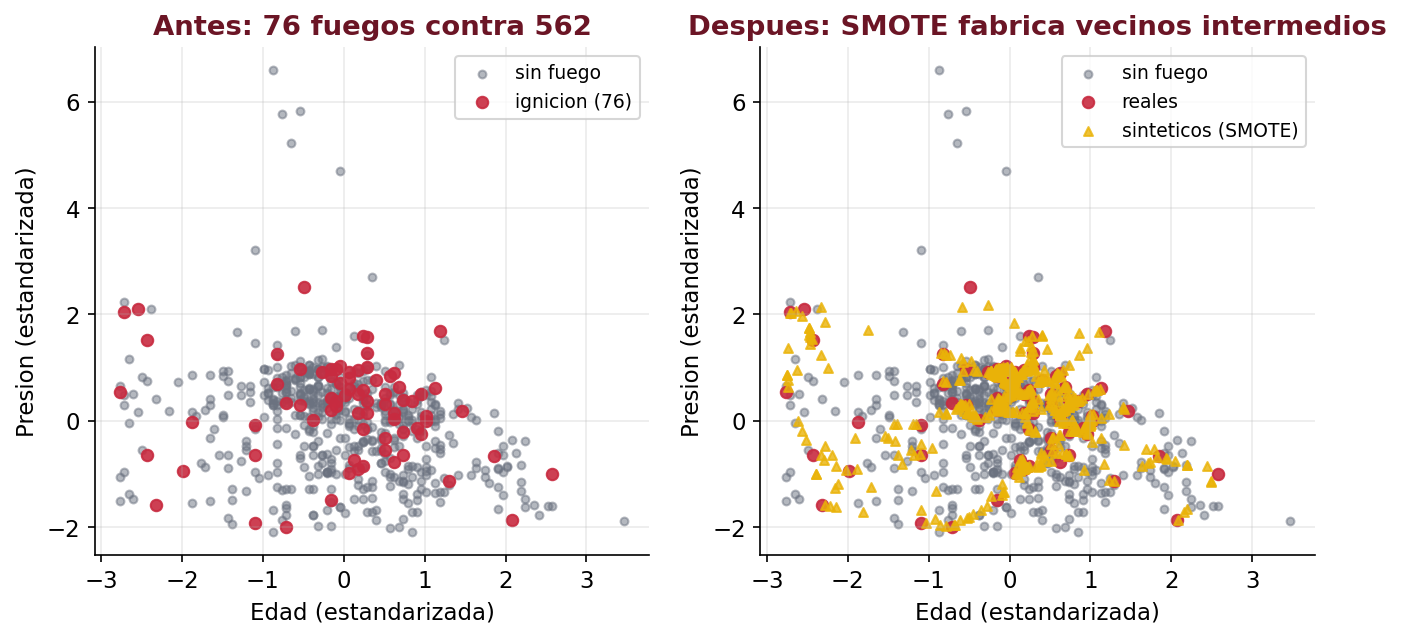
\includegraphics[height=0.55\textheight]{fig_smote.png}

  \vspace{4pt}
  {\footnotesize\color{textMuted}
  \begin{itemize}\setlength{\itemsep}{2pt}
    \item[{\color{arcaRed}\scriptsize\faArrowRight}]
      SMOTE toma cada fuego real, busca su fuego \textbf{más parecido} y crea
      puntos \textbf{intermedios} (triángulos): sintéticos pero \textbf{creíbles}.
    \item[{\color{codeGreen}\scriptsize\faCheck}]
      El train pasa de 53 fuegos a \textbf{393 contra 393}.
      Regla sagrada: \textbf{SOLO al train} --- inventar datos en el examen
      sería \textbf{otra fuga}.
  \end{itemize}
  }
\end{frame}

% ── SMOTE CÓDIGO ─────────────────────────────────────────────────────────────
\begin{frame}[fragile,shrink=26]{SMOTE en Código: una Pieza Más en el Tubo}
  \vspace{-4pt}
  {\small\color{arcaDark}\bfseries
    La librería \texttt{imblearn} trae un pipeline que sabe aplicar SMOTE solo donde toca.}

  \vspace{4pt}
  \begin{columns}[T]
    \begin{column}{0.58\textwidth}
      \begin{pyblock}
from imblearn.over_sampling import SMOTE
from imblearn.pipeline import make_pipeline

tubo_smote = make_pipeline(
    StandardScaler(),        # escalar
    SMOTE(random_state=42),  # equilibrar (solo train)
    SVC())                   # clasificar
tubo_smote.fit(X_tr, y_fuego_tr)
      \end{pyblock}
      \vspace{2pt}
      \begin{outputblock}
Pipeline(steps=[('standardscaler', ...),
                ('smote', ...), ('svc', ...)])
      \end{outputblock}
    \end{column}
    \begin{column}{0.38\textwidth}
      {\scriptsize\color{textMuted}
      \begin{itemize}\setlength{\itemsep}{5pt}
        \item[{\color{codeGreen}\scriptsize\faCheck}]
          El tubo aplica SMOTE al entrenar\ldots{} y lo
          \textbf{omite} al predecir. Exactamente la regla
          sagrada, automatizada.
        \item[{\color{arcaRed}\scriptsize\faArrowRight}]
          \texttt{!pip install imbalanced-learn}
          en Colab si hace falta (como vimos en la Clase 3).
        \item[{\color{arcaRed}\scriptsize\faLightbulb[regular]}]
          Fíjense: el pipeline dejó de ser un truco de
          comodidad y se volvió \textbf{la arquitectura} donde
          todo encaja.
      \end{itemize}
      }
    \end{column}
  \end{columns}
\end{frame}

% ── SMOTE RESULTADO ──────────────────────────────────────────────────────────
\begin{frame}{El Despertar del Modelo (y su Precio)}
  \vspace{-6pt}
  \begin{columns}[T]
    \begin{column}{0.6\textwidth}
      \centering
      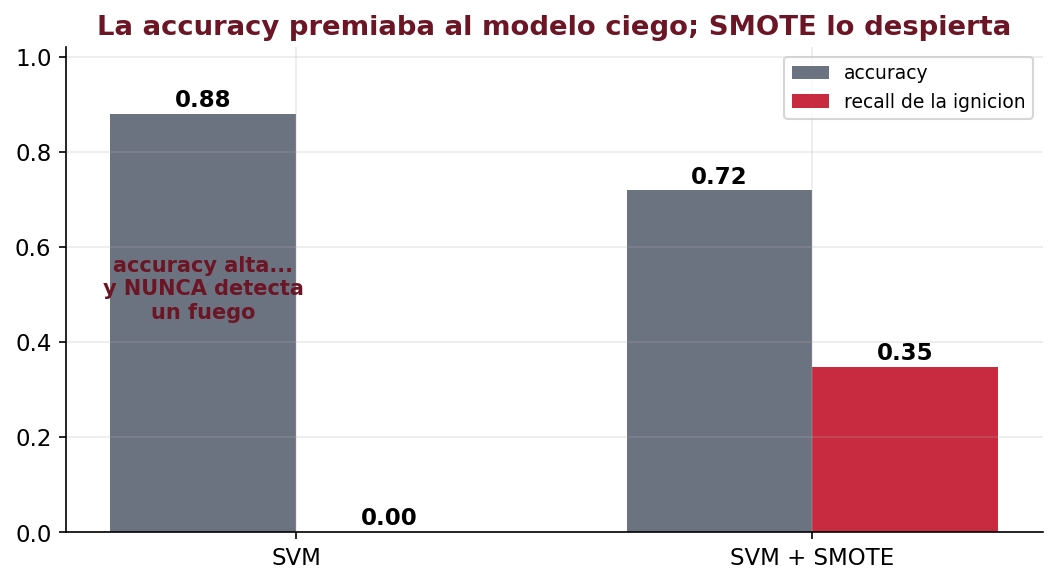
\includegraphics[width=\textwidth]{fig_smote_resultado.png}
    \end{column}
    \begin{column}{0.36\textwidth}
      {\footnotesize\color{textMuted}
      \begin{itemize}\setlength{\itemsep}{5pt}
        \item[{\color{codeGreen}\scriptsize\faCheck}]
          Recall del fuego: \textbf{0.00 \(\to\) 0.35}.
          Ahora detecta 8 de 23 fuegos del test.
        \item[{\color{arcaRed}\scriptsize\faExclamationTriangle}]
          El precio: 39 \textbf{falsas alarmas} (accuracy baja
          a 0.72; 1 de cada 5--6 alertas es fuego real).
        \item[{\color{arcaRed}\scriptsize\faBalanceScale}]
          ¿Vale la pena? Con fuego a \textbf{\$896\,000} y falsa
          alarma al costo de una \textbf{revisión preventiva},
          la cuenta sale sola. Es el trade-off del \textbf{umbral}
          de la C2, con otra herramienta.
      \end{itemize}
      }
    \end{column}
  \end{columns}
\end{frame}

% ── PRÁCTICA 2 ───────────────────────────────────────────────────────────────
\begin{frame}[shrink=8]{Su Turno: Domar el Fuego \hfill {\normalsize\color{arcaRed}\faClock\hspace{4pt}15 min}}
  \vspace{-4pt}
  {\small\color{arcaDark}\bfseries
    El SVM despertó pero paga caro. ¿Pueden conseguir un mejor trato?}

  \vspace{8pt}
  {\footnotesize
  \begin{enumerate}\setlength{\itemsep}{7pt}
    \item Armen \texttt{RandomForestClassifier} + SMOTE (con el pipeline de
      \texttt{imblearn}, sin escalador: los árboles no lo necesitan).
      Comparen accuracy y recall contra el SVM + SMOTE.
    \item Prueben \texttt{SMOTE(sampling\_strategy=0.5)} --- fabricar fuegos hasta
      la \textbf{mitad} de la clase grande, no hasta igualar. ¿Mejora el trato
      recall/falsas alarmas?
    \item Saquen la \texttt{confusion\_matrix} de su mejor opción y cuenten:
      ¿cuántos fuegos detecta? ¿cuántas falsas alarmas genera?
    \item Pregunta de negocio: con fuego = \$896\,000 y revisión preventiva =
      \$20\,000, escriban \textbf{una frase} para el gerente HSE recomendando
      (o no) desplegar su modelo.
  \end{enumerate}
  }
\end{frame}

% ═════════════════════════════════════════════════════════════════════════════
\sectionframe{Cierre del Módulo 3}{Cinco clases, un método}
% ═════════════════════════════════════════════════════════════════════════════

% ── MARCADOR ─────────────────────────────────────────────────────────────────
\begin{frame}{El Marcador Final de la Clase}
  \vspace{-6pt}
  \begin{columns}[T]
    \begin{column}{0.62\textwidth}
      \centering
      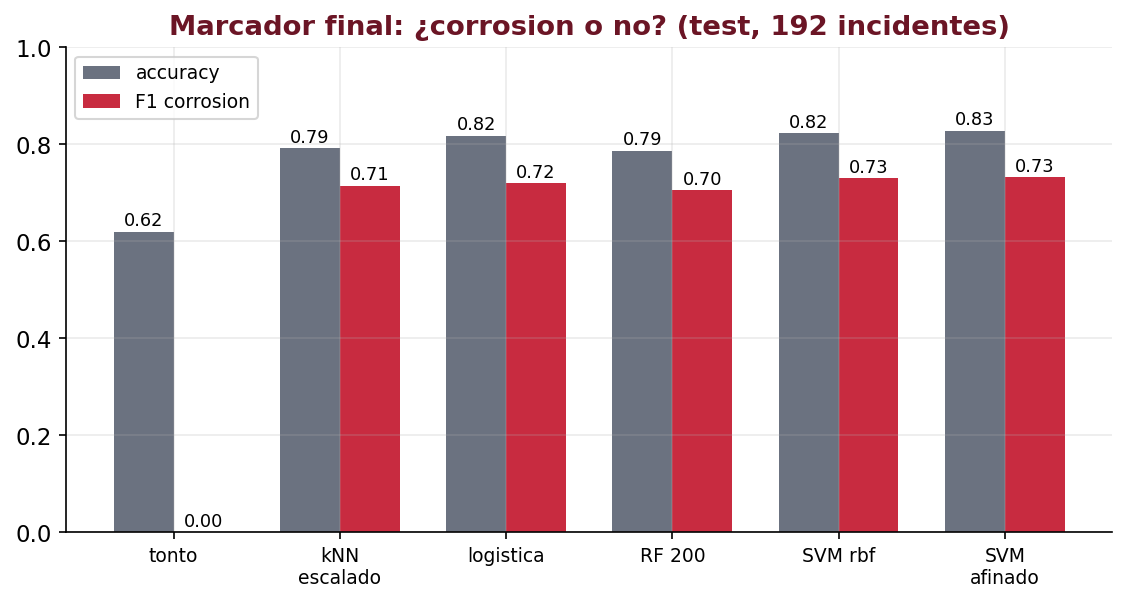
\includegraphics[width=\textwidth]{fig_marcador.png}
    \end{column}
    \begin{column}{0.34\textwidth}
      {\footnotesize\color{textMuted}
      \begin{itemize}\setlength{\itemsep}{5pt}
        \item[{\color{arcaRed}\scriptsize\faArrowRight}]
          Todos los caminos llegaron a \textbf{0.79--0.83}:
          cuando la señal es la que es, ningún modelo hace magia.
        \item[{\color{codeGreen}\scriptsize\faCheck}]
          Lo que sí cambió el juego: \textbf{escalar} (+5),
          \textbf{validar honesto} (saber que el número es real)
          y \textbf{SMOTE} (ver lo raro).
        \item[{\color{arcaRed}\scriptsize\faBullseye}]
          El método pesa más que el modelo. Ese es el cierre
          del módulo.
      \end{itemize}
      }
    \end{column}
  \end{columns}
\end{frame}

% ── MAPA DE MODELOS ──────────────────────────────────────────────────────────
\begin{frame}[shrink=12]{El Mapa de Modelos del Módulo: Cuál Usar Cuándo}
  \vspace{-4pt}
  {\footnotesize
  \begin{tabular}{@{}lp{4.6cm}p{4.6cm}c@{}}
    \toprule
    {\color{arcaDark}\bfseries Modelo} & {\color{arcaDark}\bfseries Su fuerte} &
    {\color{arcaDark}\bfseries Su debilidad} & {\color{arcaDark}\bfseries ¿Escalar?} \\
    \midrule
    Regresión lineal & explicable, rápida, un número por variable
      & solo relaciones de paso parejo & sí \\
    Logística & igual, pero para clasificar; da probabilidades
      & fronteras rectas & sí \\
    Árbol & se dibuja y se explica solo & inestable, memoriza fácil & no \\
    Random Forest & potente sin afinar casi nada & caja más oscura, pesado
      & no \\
    SVM & margen máximo; kernel para lo curvo & lenta con muchos datos;
      C y gamma & \textbf{sí, siempre} \\
    \bottomrule
  \end{tabular}
  }

  \vspace{8pt}
  {\footnotesize\color{textMuted}
  \begin{itemize}\setlength{\itemsep}{3pt}
    \item[{\color{arcaRed}\scriptsize\faArrowRight}]
      Receta profesional: empiecen por el \textbf{simple} (logística / lineal),
      luego \textbf{Random Forest}, y SVM cuando el problema lo pida.
      Comparen \textbf{siempre} contra el tonto.
    \item[{\color{arcaRed}\scriptsize\faForward}]
      Para su radar (no lo vimos): \emph{gradient boosting} (XGBoost) ---
      el primo competitivo del bosque --- y \emph{k-NN}, el clasificador por
      vecinos. Con lo de hoy pueden aprenderlos solos.
  \end{itemize}
  }
\end{frame}

% ── RESUMEN CLASE ────────────────────────────────────────────────────────────
\begin{frame}[shrink=10]{Lo Que Aprendimos Hoy}
  \vspace{-4pt}
  \begin{columns}[T]
    \begin{column}{0.48\textwidth}
      {\footnotesize\color{arcaDark}\bfseries Conceptos}
      \vspace{3pt}
      {\footnotesize\color{textMuted}
      \begin{itemize}\setlength{\itemsep}{2pt}
        \item[{\color{codeGreen}\scriptsize\faCheck}]
          SVM: la carretera más ancha (margen, vectores de soporte)
        \item[{\color{codeGreen}\scriptsize\faCheck}]
          Kernel trick: subir de dimensión sin pagar el costo
        \item[{\color{codeGreen}\scriptsize\faCheck}]
          Pipeline: honestidad automatizada
        \item[{\color{codeGreen}\scriptsize\faCheck}]
          Validación cruzada: 5 fotos mienten menos
        \item[{\color{codeGreen}\scriptsize\faCheck}]
          Fuga de información: sus 3 disfraces
        \item[{\color{codeGreen}\scriptsize\faCheck}]
          GroupKFold: ¿el modelo viaja? (facies: no viajaba)
        \item[{\color{codeGreen}\scriptsize\faCheck}]
          SMOTE: fabricar lo raro, solo en el train
      \end{itemize}
      }
    \end{column}
    \begin{column}{0.48\textwidth}
      {\footnotesize\color{arcaDark}\bfseries Herramientas}
      \vspace{3pt}
      {\footnotesize\color{textMuted}
      \begin{itemize}\setlength{\itemsep}{2pt}
        \item[{\color{arcaRed}\scriptsize\faTools}]
          \texttt{SVC} (\texttt{kernel}, \texttt{C}, \texttt{gamma})
        \item[{\color{arcaRed}\scriptsize\faTools}]
          \texttt{make\_pipeline}, \texttt{StandardScaler}
        \item[{\color{arcaRed}\scriptsize\faTools}]
          \texttt{cross\_val\_score}, \texttt{GroupKFold}
        \item[{\color{arcaRed}\scriptsize\faTools}]
          \texttt{GridSearchCV} con \texttt{svc\_\_C}
        \item[{\color{arcaRed}\scriptsize\faTools}]
          \texttt{SMOTE} + pipeline de \texttt{imblearn}
      \end{itemize}
      }
      \vspace{8pt}
      \begin{tcolorbox}[colback=arcaGray, colframe=arcaRed, boxrule=0pt, leftrule=3pt,
        arc=3pt, left=6pt, right=6pt, top=5pt, bottom=5pt]
        {\scriptsize\color{arcaDark}\bfseries El número del día:}\\[3pt]
        {\scriptsize\color{textMuted}
          facies con pozos por fuera: \textbf{0.78 \(\to\) 0.53}.
          El espejismo medía \textbf{25 puntos} --- y solo la
          validación honesta lo vio.}
      \end{tcolorbox}
    \end{column}
  \end{columns}
\end{frame}

% ── ARCO DEL MÓDULO ──────────────────────────────────────────────────────────
\begin{frame}[shrink=8]{El Arco Completo del Módulo 3}
  \vspace{-4pt}
  {\small\color{arcaDark}\bfseries
    Cinco clases, y en cada una la misma pregunta: ¿qué decisión habilita este modelo y cuánto cuesta equivocarse?}

  \vspace{10pt}
  {\footnotesize\color{textMuted}
  \begin{itemize}\setlength{\itemsep}{6pt}
    \item[{\color{arcaRed}\bfseries C1}]
      Predecir un \textbf{número} (regresión) --- el sónico de Volve, R\(^2\), residuos
    \item[{\color{arcaRed}\bfseries C2}]
      Predecir una \textbf{etiqueta} (logística) --- litología, métricas,
      \textbf{costo de negocio} y umbral
    \item[{\color{arcaRed}\bfseries C3}]
      Romper la recta (\textbf{árboles y bosque}) --- las lunas, overfitting,
      el récord de costo
    \item[{\color{arcaRed}\bfseries C4}]
      Elegir entre \textbf{muchas} (multiclase) --- facies, codificar, imputar,
      macro/weighted, penalización
    \item[{\color{arcaRed}\bfseries C5}]
      Hacerlo \textbf{honesto} (SVM, pipeline, CV, GroupKFold, SMOTE) ---
      ductos, fuego, y la verdad sobre el 0.78
  \end{itemize}
  }

  \vspace{8pt}
  \centering
  {\footnotesize\color{arcaDark}\itshape
    Ya no son personas que corren \texttt{.fit()}: son ingenieros que saben
    \textbf{cuándo creerle a un modelo}.}
\end{frame}

% ── GRACIAS ──────────────────────────────────────────────────────────────────
\begingroup
\setbeamertemplate{headline}{}
\setbeamertemplate{footline}{}
\setbeamertemplate{navigation symbols}{}
\begin{frame}[plain, noframenumbering]
  \begin{tikzpicture}[remember picture, overlay]
    \fill[arcaDark] (current page.south west) rectangle (current page.north east);
    \node[anchor=center, text=white, font=\Huge\bfseries]
      at ([yshift=1.5cm]current page.center) {¡Gracias!};
    \node[anchor=center, text=white!80, font=\large, text width=10cm, align=center]
      at ([yshift=0.2cm]current page.center)
      {Carlos Enrique Mosquera Trujillo};
    \node[anchor=center, text=white!60, font=\normalsize, text width=10cm, align=center]
      at ([yshift=-0.6cm]current page.center)
      {\faEnvelope\hspace{6pt}cmosquerat@unal.edu.co};
    \node[anchor=center, text=white!60, font=\normalsize, text width=11cm, align=center]
      at ([yshift=-1.3cm]current page.center)
      {Machine Learning for Petroleum Engineers Using Python};
    \node[anchor=center, text=white!40, font=\small]
      at ([yshift=-2.0cm]current page.center)
      {Fin del Módulo 3 \quad$\cdot$\quad SLB Ecuador \quad$\cdot$\quad UDLA \quad$\cdot$\quad 2026};
  \end{tikzpicture}
\end{frame}
\endgroup

\end{document}
